\documentclass[11pt, a4paper]{article}
\usepackage{graphicx}
\usepackage{amssymb}
\usepackage{amsmath}
\usepackage{mathtools}
\usepackage{wrapfig}
\usepackage{dsfont}
\usepackage{lipsum}  
\usepackage{float}
\usepackage{color}

\DeclareGraphicsRule{.tif}{png}{.png}{`convert #1 `basename #1 .tif`.png}

\textwidth = 6.5 in
\textheight = 9 in
\oddsidemargin = 0.0 in
\evensidemargin = 0.0 in
\topmargin = 0.0 in
\headheight = 0.0 in
\headsep = 0.0 in
\parskip = 0.0in
\parindent = 0.2in
\linespread{1.3}

\def\dul#1{\underline{\underline{#1}}}
\def\ul#1{\underline{#1}}
\def\frvecop#1{\hat{\tilde{\underline{#1}}}}
\def\frmat#1{\tilde{\dul{#1}}}
\def\myeq#1{\stackrel{\mathclap{\tiny\mbox{#1}}}{=}}
\def\frop#1{\hat{\tilde{#1}}}

\def\ket#1{|#1\rangle}
\def\e#1{ e^{#1}}
\def\bra#1{\langle#1|}
\def\av#1{\langle#1\rangle}

\def\tder#1{\frac{d#1}{dt}}
\def\eps{\varepsilon}
\def\nup{\nu^\prime}

\def\aop{\hat{a}}
\def\adop{\hat{a}^\dagger}
\def\dop{\hat{d}}
\def\ddop{\hat{d}^\dagger}
\def\sigop{\hat{\sigma}^-}
\def\sigdop{\hat{\sigma}^+}
\def\Hop{\hat{H}}
\def\Hpop{\hat{H}^\prime}
\def\qp{{q^\prime}}
\def\tp{{t^\prime}}
\def\kappap{{\kappa^\prime}}

\def\thetap{\theta^\prime}

\def\ctil{\tilde{c}}
\def\nn{\nonumber}

\newcommand{\lsz}{\left[}
\newcommand{\rsz}{\right]}
\newcommand{\lk}{\left(}
\newcommand{\rk}{\right)}
\newcommand{\lka}{\left\{}
\newcommand{\rka}{\right\}}
\newcommand{\labs}{\left|}
\newcommand{\rabs}{\right|}
\newcommand{\lla}{\left\langle}
\newcommand{\rra}{\right\rangle}

\usepackage{hyperref}
\def\refeq#1{{\hyperref[#1]{(\ref*{#1})}}}
\def\reffig#1{{\hyperref[#1]{FIG. \ref*{#1}}}}
\def\refsec#1{{\hyperref[#1]{SEC. \ref*{#1}}}}
\def\refno#1{{\hyperref[#1]{\ref*{#1}}}}

\title{Cavity QED with a feedback via a perfectly reflecting mirror}
\author{Nikolett Nemet, Scott Parkins and Andreas Knorr}
\begin{document}
\maketitle
\section{Setup}
In our investigation we look at a closed system, or from another perspective an open cavity-qed system, where its output field is fed back by a perfectly reflecting mirror at a distance L. In \reffig{fig:setup} the basic schematic setup is depicted.

\begin{figure}[h!]
\centering
%\vglue -.2 cm
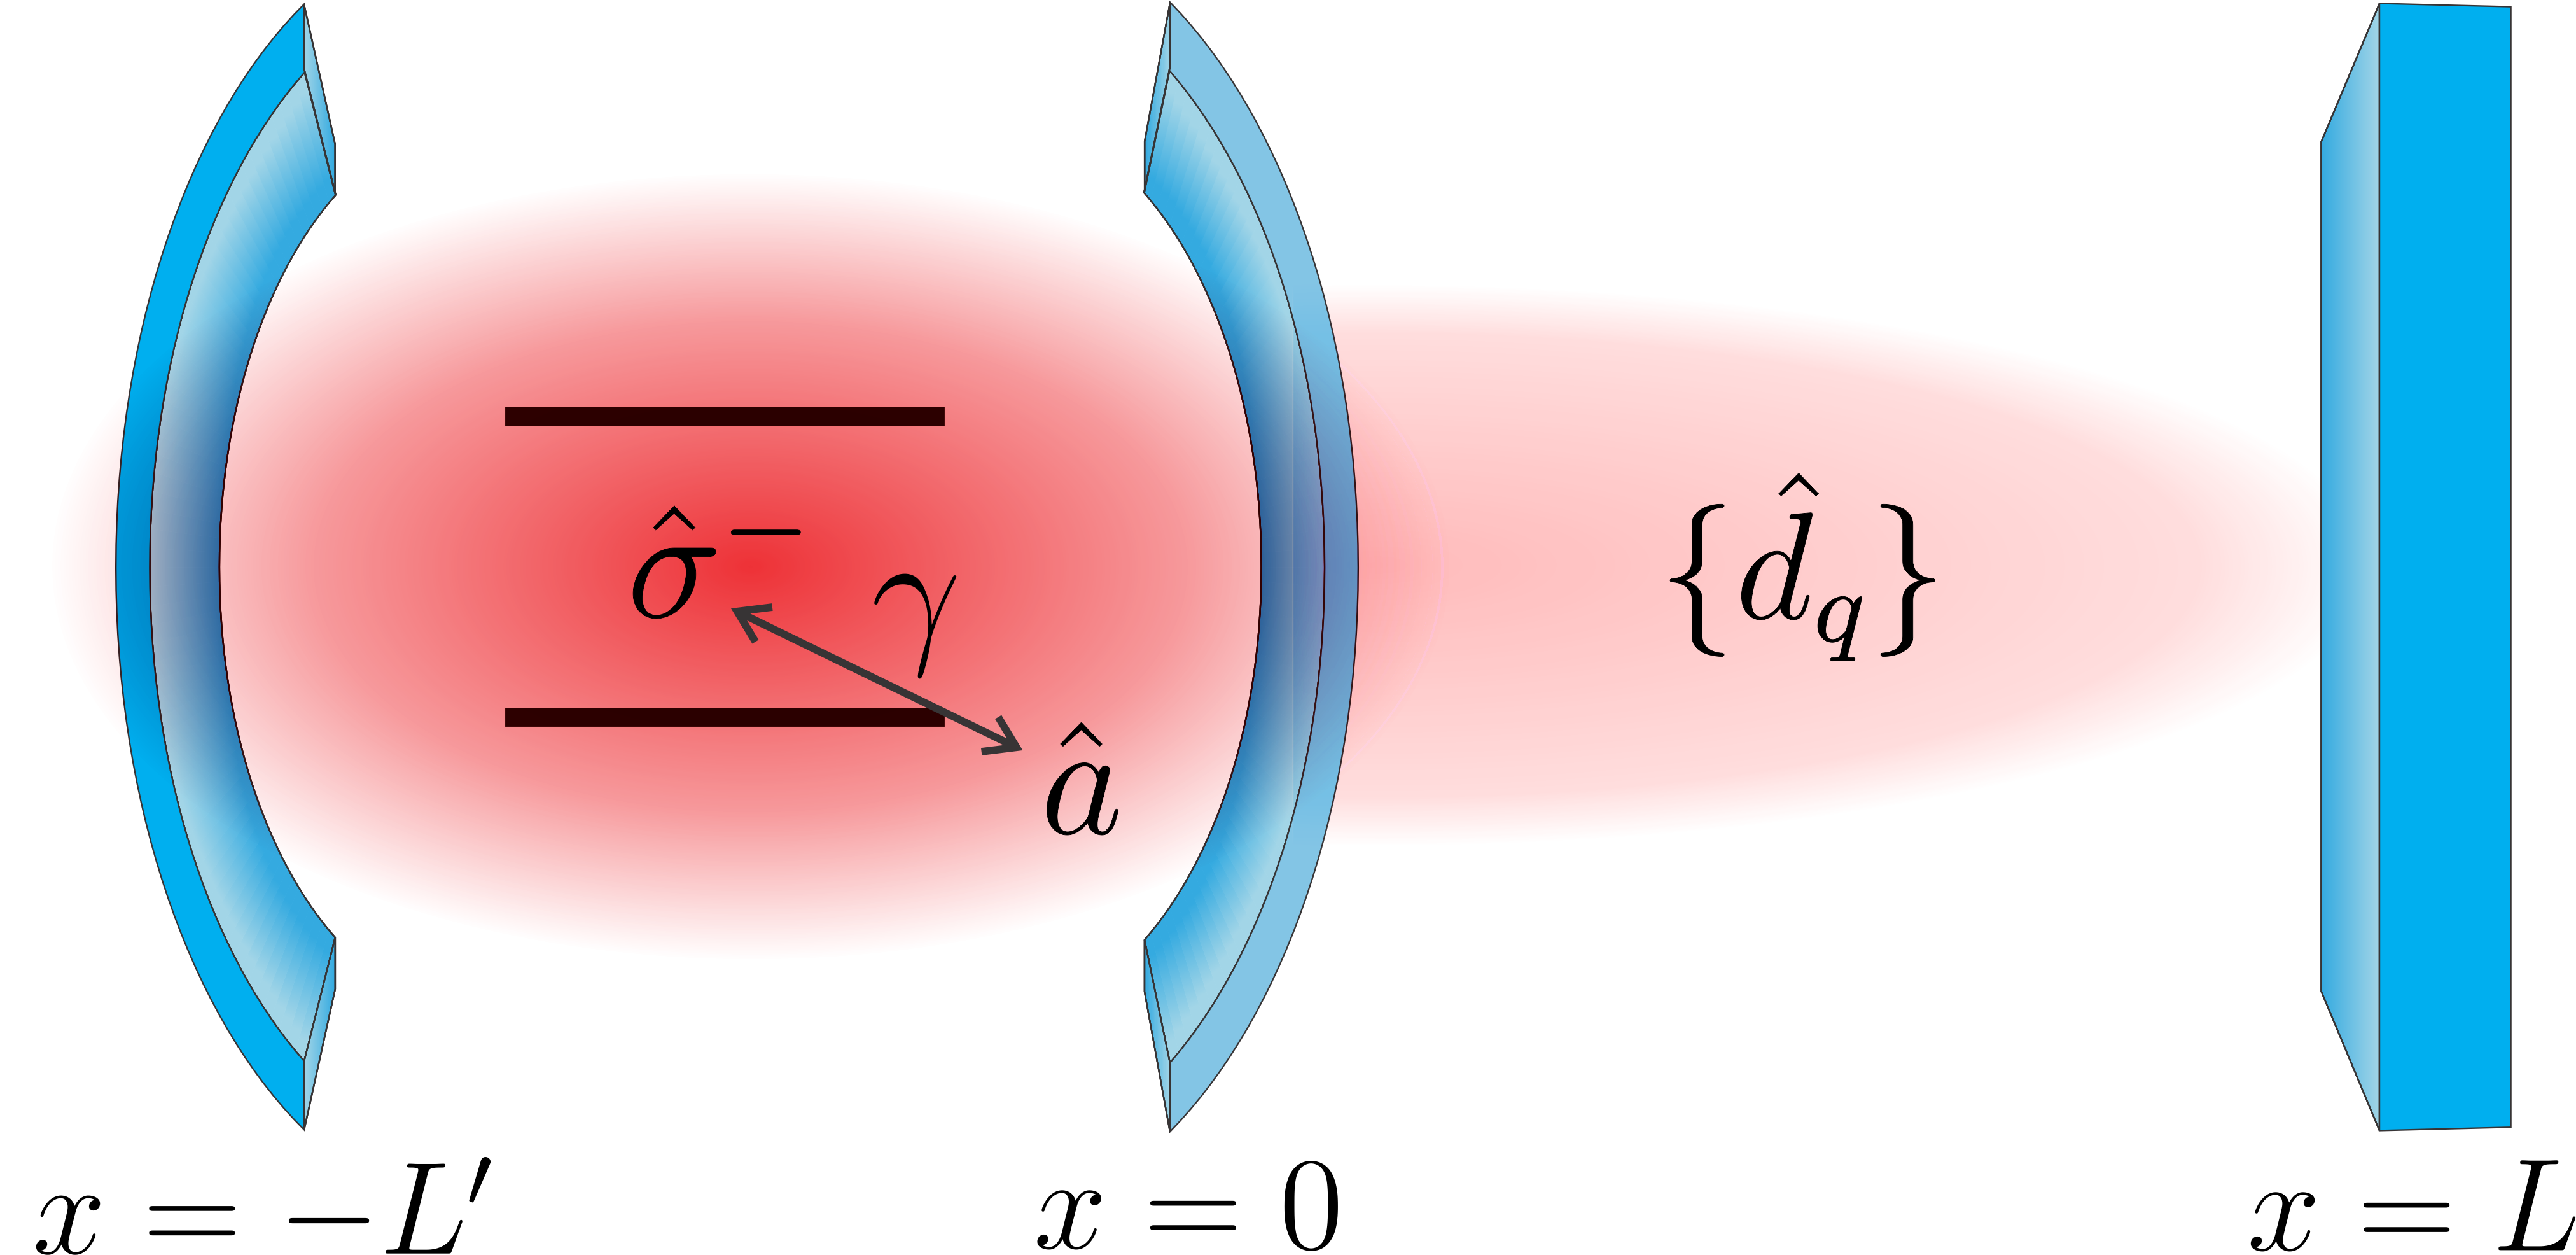
\includegraphics[width=.45\textwidth]{Setup.png}
\vglue -0.8 cm
\label{fig:setup}
\textit{\textbf{\caption{\linespread{1}\small{Schematic setup. The one-sided cavity contains a two-level system with resonance frequency $\omega_a$. The coupling strength between the cavity mode with frequency $\omega_c$ and the external modes of frequency $\omega_q$ are frequency-dependent and can be described by $G_q(t)$.}}}}
\vglue -.3 cm
\end{figure}

\noindent In order to avoid a multimode treatment of the cavity, we focus on the case, when $L^\prime\ll L$.
\section{Theoretical model}
\subsection{System Hamiltonian}
The Hamiltonian of such a system in the rotating-wave and dipole approximations has the following form:
\begin{align}
\Hop_0 &= \hbar\omega_a\sigdop\sigop + \hbar\omega_c\adop\aop + \frac{\pi}{L}\sum_{q=0}^\infty\hbar\omega_q\ddop_q\dop_q\nn\\
\Hop &= \Hop_0 - \hbar\gamma\lk\adop\sigop + \sigdop\aop\rk - \frac{\pi}{L}\sum_{q=0}^\infty\lk\hbar G_q\adop\dop_q + \hbar G^*_q\ddop_q\aop\rk\nn
\end{align}
where $\gamma$ is the coupling strength between the two-level transition and the cavity mode. The mode spacing of the external field $\pi/L$ is there, because we consider unnormalized modes in $\dop_q$. This Hamiltonian is similar to what was published in \cite{Kabuss2015}. There an originally non-structured reservoir was considered with continuous frequency spectrum. The perfectly reflecting mirror served as a boundary condition influencing only the coupling strength of the two spaces. In our case, the mirror as a boundary condition defines the external standing-wave modes with quantized frequencies as well as its coupling to the cavity via these modes, therefore this model can consider shorter lengths in $L$. Practically that external part of the system serves as a second, larger multimode cavity, the mode-functions of which can be expressed as (with the perfectly reflecting mirror at $x=L$):
\begin{align}
u_q(x) &= \sin{\lsz k_q(x-L)\rsz},\nn\\
k_q &=\frac{(2q+1)\pi}{2L},\  q\in\mathbb{N},\nn\\
\omega_q & = c_0k_q.
\end{align}

The interaction strength has the following form at the coupling mirror $(x=0)$:
\begin{align}
G_q = G_0\sin{(k_qL)}.
\end{align}
This coupling is similar to the one in \cite{Kabuss2015,Dorner2002}. Our system is different compared to the case considered in \cite{Dorner2002} in that the cavity mirror closer to the external mirror has a high reflectivity in a wide range of frequencies, which supports the creation of standing wave modes with specific frequencies more than a single atom. 

Now let us consider our system in the interaction frame described by $\Hop_0$, where the frequency of the cavity mode is tuned to the atomic resonance $\lk \omega_a=\omega_c=\omega_0\rk$:
\begin{align}
\Hpop &= -\hbar\gamma\lk\adop\sigop + \sigdop\aop\rk - \frac{\pi}{L}\sum_{q=0}^\infty\lk\hbar G_q(t)\adop\dop_q + \hbar G^*_q(t)\ddop_q\aop\rk,\nn\\
G_q(t) &= G_0\sin{(k_qL)}e^{i(\omega_0-\omega_q)t} = G_0\sin{\lsz(k_\qp+k_0)L\rsz}e^{-i\omega_\qp t} = G_\qp(t),
\end{align}
where $G_0$ is the tunnel coupling strength introduced in \cite{Kabuss2015}. We also introduced the shifted frequency $\omega_\qp$, which is centered closely around the cavity resonance as:
\begin{align}
\label{omega_qp_def}
\omega_\qp = \frac{\qp\pi c_0}{L}+\Delta \text{, where } \qp\in\mathbb{Z}, \Delta<\frac{\pi}{L}c_0.
\end{align}
As the cavity frequency is much larger than the mode spacing of the individual external modes, the lower boundary of the sum can be shifted to $-\infty$, thus
\begin{align}
\Hpop = -\hbar\gamma\lk\adop\sigop + \sigdop\aop\rk - \frac{\pi}{2L}\sum_{\qp=-\infty}^\infty\lk\hbar G_{\qp}(t)\adop\dop_{\qp} + \hbar G^*_{\qp}(t)\ddop_{\qp}\aop\rk,
\end{align}
where we added a factor of $1/2$ as with this symmetric mode distribution there are twice the number of modes and the contribution of the "negative" frequencies is the same as the positive ones.

\subsection{Equations of motion in the single-excitation manifold}
The perfectly reflecting mirror at distance $L$ can be considered as a mean of feedback of the output of the cavity. The corresponding time-delay in the feedback loop is
\begin{align}
\label{tau_def}
\tau = \frac{2L}{c_0},
\end{align}
and in this way non-Markovian dynamics is enforced. This means that the system cannot be investigated analytically outside the one-excitation manifold. The wave-function in this case can be expressed as
\begin{align}
\ket{\psi(t)} = c_e(t)\ket{e,0,\{0\}} + c_g(t)\ket{g,1,\{0\}} + \frac{\pi}{2L}\sum_\qp c_{g,\qp}(t)\ket{g,0,\{\qp\}}.
\end{align}
The Schr\"odinger equation provides the equations of motion for these amplitudes:
\begin{align}
\label{c_e_eq}
\frac{dc_e}{dt} &= i\gamma c_g(t),\\
\label{c_g_eq}
\frac{dc_g}{dt} &= i\gamma c_e(t) + i\frac{\pi}{2L}\sum_{\qp=-\infty}^{\infty}G_\qp(t)c_{g,\qp}(t),\\
\label{c_gqp_eq}
\frac{dc_{g,\qp}}{dt} &= iG^*_\qp(t)c_g(t).
\end{align}
Substituting back the formal integral of \refeq{c_gqp_eq} gives for \refeq{c_g_eq}:
\begin{align}
\frac{dc_g}{dt} &= i\gamma c_e(t) - \frac{|G_0|^2\pi}{2L}\sum_{\qp=-\infty}^{\infty}\sin^2{\lsz(k_\qp+k_0)L\rsz}\int_0^te^{-i\omega_\qp (t-\tp)} c_{g}(\tp)d\tp\nn.
\end{align}
Let us evaluate the different parts of the expression above by using \refeq{omega_qp_def} and \refeq{tau_def}:
\begin{align}
\sin^2{\lsz(k_\qp+k_0)L\rsz} &= \sin^2{\lsz\lk\omega_\qp+\omega_0\rk\frac{\tau}{2}\rsz} =
 -\frac{1}{4}\lsz e^{i2\qp\pi}e^{i\lk\omega_0+\Delta\rk\tau}+e^{-i2\qp\pi}e^{-i\lk\omega_0+\Delta\rk\tau}-2 \rsz=\nn\\
&=\frac{1-\cos{\lsz\lk\omega_0+\Delta\rk\tau\rsz}}{2} = \sin^2{\lsz\frac{\omega_0+\Delta}{2}\tau\rsz}.
\end{align}
Thus this part is not dependent on frequency, therefore we can evaluate the rest separately
\begin{align}
\sum_{\qp=-\infty}^{\infty}e^{-i\omega_\qp (t-\tp)} = e^{-i\Delta (t-\tp)}\sum_{\qp=-\infty}^{\infty}e^{-i\qp 2\pi \frac{t-\tp}{\tau}} = 
\tau e^{-i\Delta (t-\tp)}\sum_{\qp = -\infty}^\infty\delta\lk t-\tp-\qp\tau\rk,
\end{align}
where we have used the Fourier series identity for the Dirac comb. Putting everything together gives:
\begin{align}
\frac{dc_g}{dt} &= i\gamma c_e(t) - \frac{|G_0|^2\pi\tau}{2L}\sin^2{\lsz\frac{\omega_0+\Delta}{2}\tau\rsz}\sum_{\qp=-\infty}^{\infty}\int_0^t\delta\lk t-\tp-\qp\tau\rk e^{-i\Delta(t-\tp)} c_{g}(\tp)d\tp.\nn
\end{align}
The integration range excludes the case, when $\qp<0$,also for $\qp=0$ it only involves "half" of the Dirac-delta, therefore
\begin{align}
\frac{dc_g}{dt} &= i\gamma c_e(t) - \underbrace{\frac{|G_0|^2\pi}{c_0}\sin^2{\lsz\frac{\omega_0+\Delta}{2}\tau\rsz}}_{4\kappap}\lka\sum_{\qp=0}^{\infty}e^{i\Delta\qp\tau} c_{g}(t-\qp\tau)\Theta(t-\qp\tau)-\frac{1}{2}c_g(t)\rka,
\end{align}
which means, that the history of the amplitudes should be included at multiple times.

From now on I will assume, that $\Delta=0$. Then, if $\omega_0\tau=n 2\pi\ (n\in\mathbb{N})$, - which means that the external modes serve as a resonant cavity - the whole dynamics reduces to a simple cavity-QED. This makes sense, as in this case the resonant field has no contribution at the coupling mirror because of the boundary conditions at the perfectly reflecting mirror. For the sake of simplicity, we assume $\omega_0\tau=\pi$. 

\section{Poles of the Laplace Transform}
The equations of Laplace Transforms corresponding to the equations of motion with an initially excited atom have the following form:
\begin{align}
\label{eq:lap_ce}
s\ctil_e(s) &= 1+i\gamma\ctil_g(s)\\
\label{eq:lap_cg}
s\ctil_g(s) &= i\gamma\ctil_e(s) - 4\kappap\ctil_g(s)\lsz\sum_\qp e^{-s\qp\tau}-\frac{1}{2}\rsz
\end{align}

\subsection{$t<\tau$}
For short times we get back the solution without feedback:
\begin{align}
\ctil_g^{(0)}(s) = \frac{i\gamma}{s^2+\gamma^2+2\kappap s}
\end{align}
with poles at 
\begin{align}
-\kappap\pm i\gamma\sqrt{1-\frac{\kappap^2}{\gamma^2}}
\end{align}
that gives a time-dependent solution
\begin{align}
c_g^{(0)}(t) = i\gamma\frac{\sin{\lsz\sqrt{1-\frac{\kappap^2}{\gamma^2}}\gamma t\rsz}}{\sqrt{1-\frac{\kappap^2}{\gamma^2}}}e^{-\kappap t},
\end{align}
which means damped oscillations with a shifted frequency both depending on the coupling strength between the cavity and the external modes.

\subsection{Long-time limit}
In general the solution at $n\tau\le t<(n+1)\tau$ looks like
\begin{align}
\ctil_g^{(n)}(s) = \frac{i\gamma}{s^2+\gamma^2-2\kappap s+4\kappap s\sum_{\qp=0}^{n}e^{-s\qp\tau}}.
\end{align}
Looking at the poles on the complex plane, which determine the dynamics, is it possible to recover Rabi oscillations with frequency $\gamma$ without any damping or frequency shift as reported in \cite{Kabuss2015}? Formally, it means that $s_R=\pm i\gamma$. This can be investigated by substituting $s_R$ back and setting the denominator to 0, which gives
\vspace{-.4cm}
\begin{align}
\sum_{\qp=0}^ne^{\mp i\gamma\qp\tau} = \frac{1}{2}.
\end{align}
In the long time limit, the left-hand side turns into an infinite geometric series. However the absolute value of the individual terms are 1, which means that the sum diverges. Thus no time-delay can satisfy this requirement.

\vspace{-.2cm}
\section{Results}
\subsection{Parameters used in \cite{Kabuss2015}}

In this case the distance of the perfectly reflecting mirror is always adjusted as to have 
$$\tau=\frac{2\pi}{\gamma}.$$
\begin{figure}[h!]
\centering
\vglue -0.9 cm
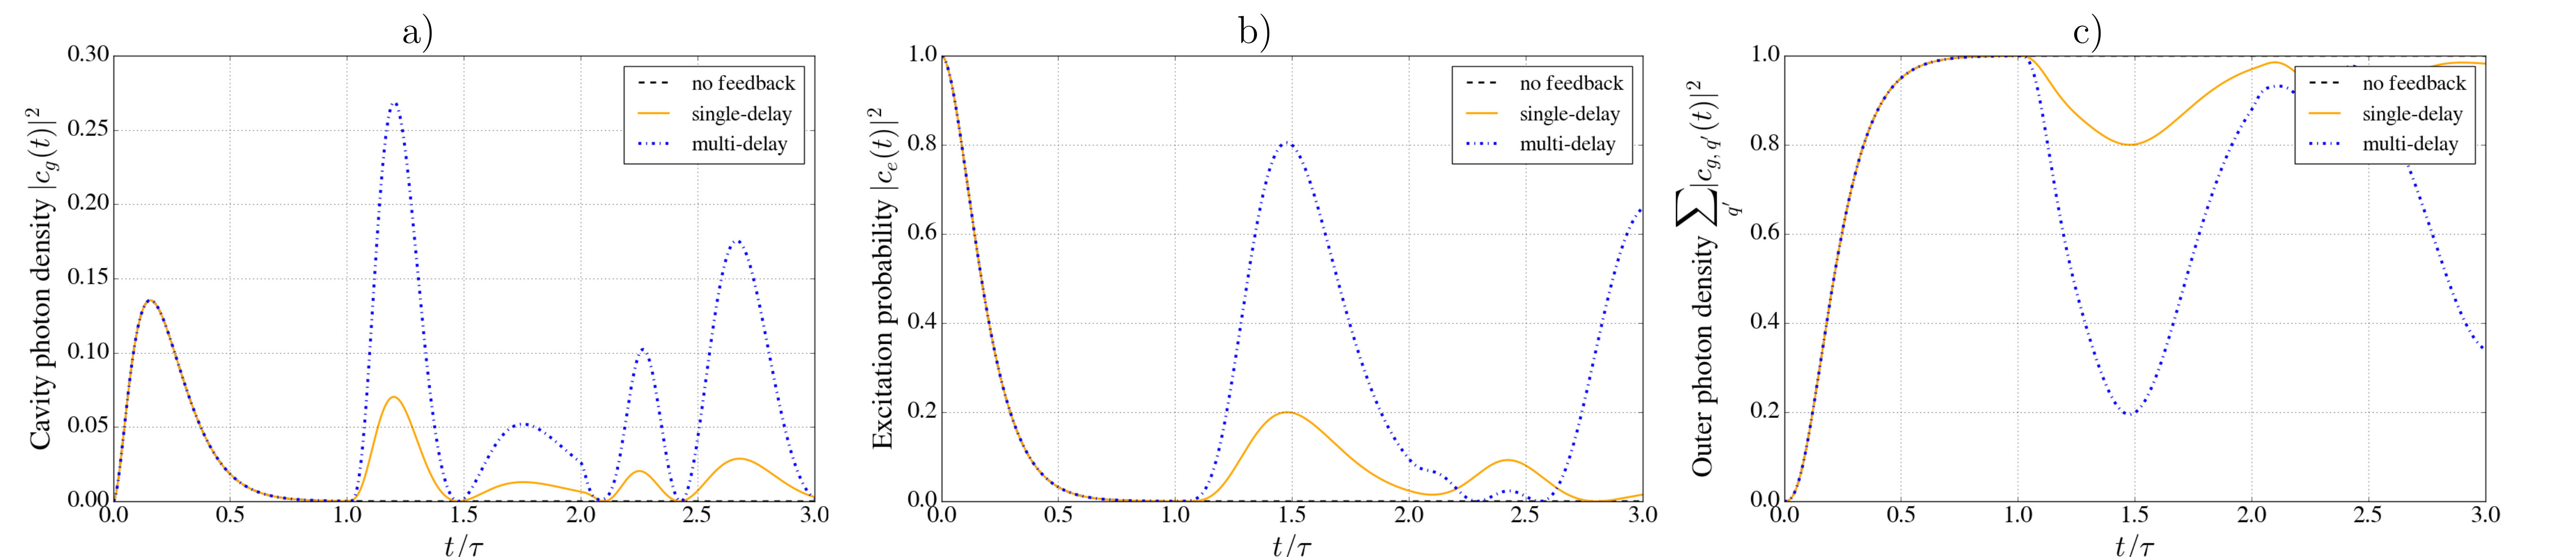
\includegraphics[width=1.05\textwidth]{shorttime_kap=2,gam=1,tau=2pi}
\vglue -1 cm
\label{fig:shortgam1_prev}
\textit{\textbf{\caption{\linespread{1}\small{Time-evolution of different excitation probabilities, when $\gamma=\kappap$ for short times. The single-delay case is calculated from \cite{Kabuss2015}.}}}}
\vglue -.3 cm
\end{figure}
\begin{figure}[h!]
\centering
\vglue -.4 cm
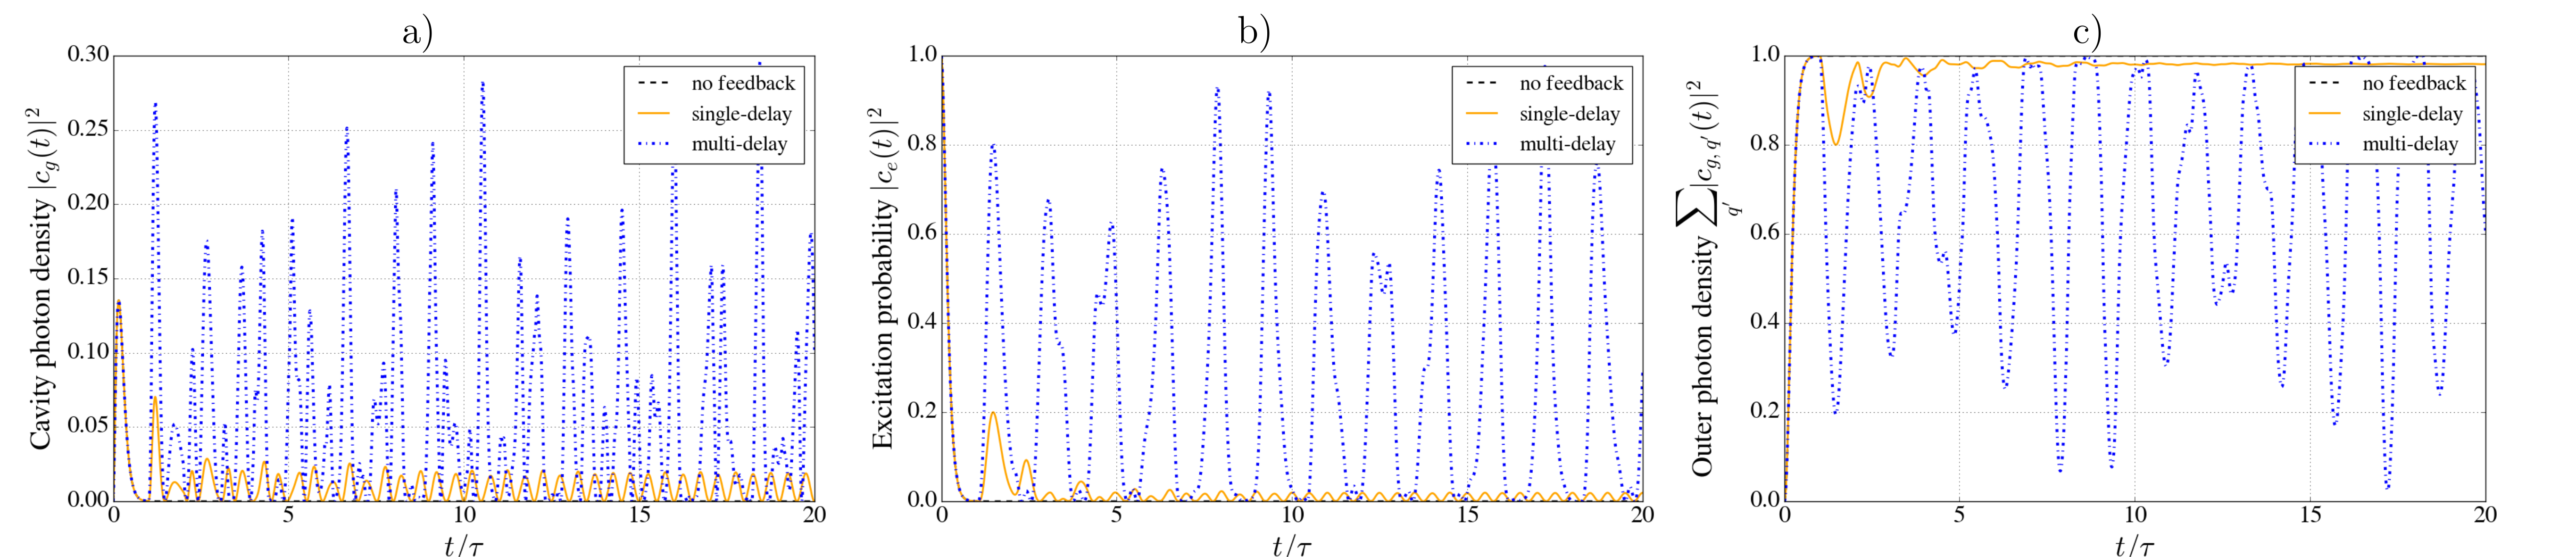
\includegraphics[width=1.05\textwidth]{longtime_kap=2,gam=1,tau=2pi}
\vglue -1 cm
\label{fig:longgam1_prev}
\textit{\textbf{\caption{\linespread{1}\small{Time-evolution of different excitation probabilities, when $\gamma=\kappap$ in the long-time limit. The single-delay case is calculated from \cite{Kabuss2015}.}}}}
\vglue -.3 cm
\end{figure}

\noindent In case of multiple delays, Rabi oscillations are not recovered in the weak coupling limit.
\enlargethispage{1cm}

\begin{figure}[h!]
\centering
\vglue .2 cm
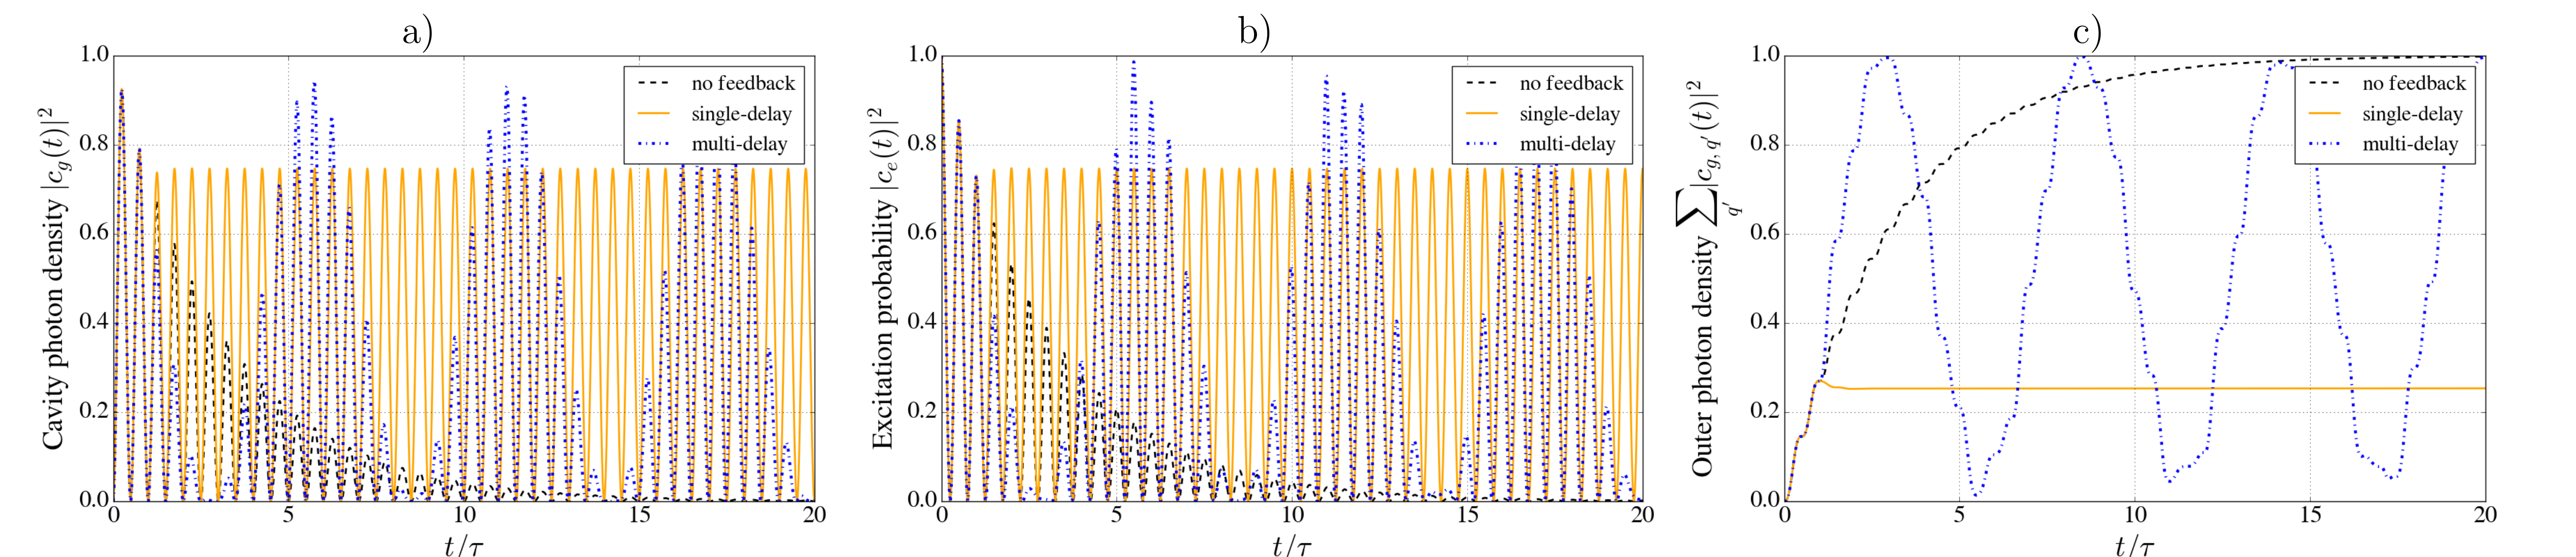
\includegraphics[width=1.05\textwidth]{longtime_kap=2,gam=40,tau=2pip40}
\vglue -1 cm
\label{fig:longgam40_prev}
\textit{\textbf{\caption{\linespread{1}\small{Time-evolution of different excitation probabilities, when $\gamma=40\kappap$ in the long-time limit. The single-delay case is calculated from \cite{Kabuss2015}.}}}}
\vglue -.3 cm
\end{figure}
\newpage

\noindent In case of strong coupling, multiple revivals can be observed in this parameter range instead of infiinite Rabi oscillations. 
\subsection{Weak-coupling regime}
When $\gamma=\kappap$, the time-evolution of the system can be expressed by using the same tricks as in \cite{Kabuss2015}:
\begin{align}
\label{eq:analytic}
c_g^{(\infty)}(t) = i\sum_{m=0}^\infty\sum_{l=0}^m\sum_{p=0}^\infty(-4)^m\frac{m(p+m-1)!}{p!l!(m-l)!}\frac{\lsz\kappap(t-p\tau)\rsz^{m+l+1}}{(m+l+1)!}e^{\kappap(t-p\tau)}\Theta(t-p\tau)
\end{align}

\enlargethispage{1cm}
\begin{figure}[h!]
\centering
\vglue -.55 cm
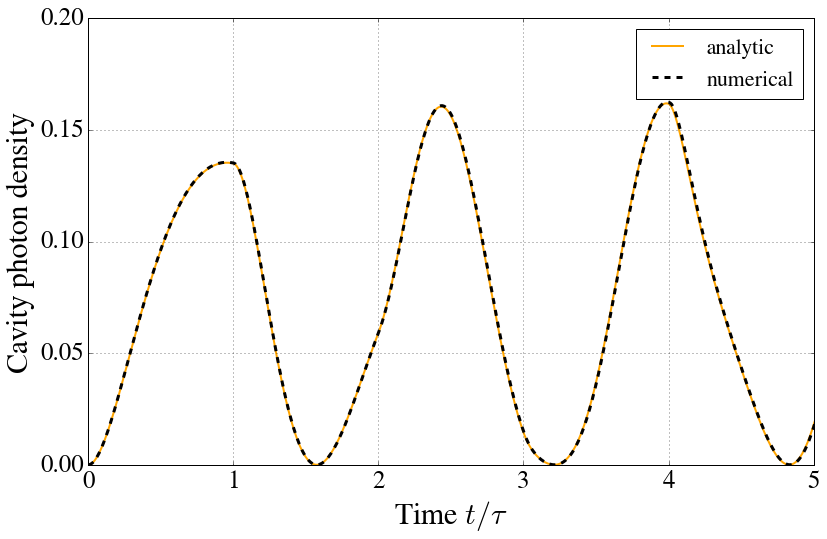
\includegraphics[width=0.57\textwidth]{cav_num,ana.png}
\vglue -1.1 cm
\label{fig:shortgam1_prev}
\textit{\textbf{\caption{\linespread{1}\small{Comparison of analytic (from \refeq{eq:analytic}) and numerical evaluation of the cavity photon density $|c_g(t)|^2$. Parameters: $\gamma=\kappap, \tau=\pi/3\gamma$}}}}
\vglue -.1 cm
\end{figure}

After finding an appropriate value of the time-delay, coherent cavity-assisted excitation exchange can be observed between the two-level system and the external modes
\begin{figure}[h!]
\centering
\vglue -.3 cm
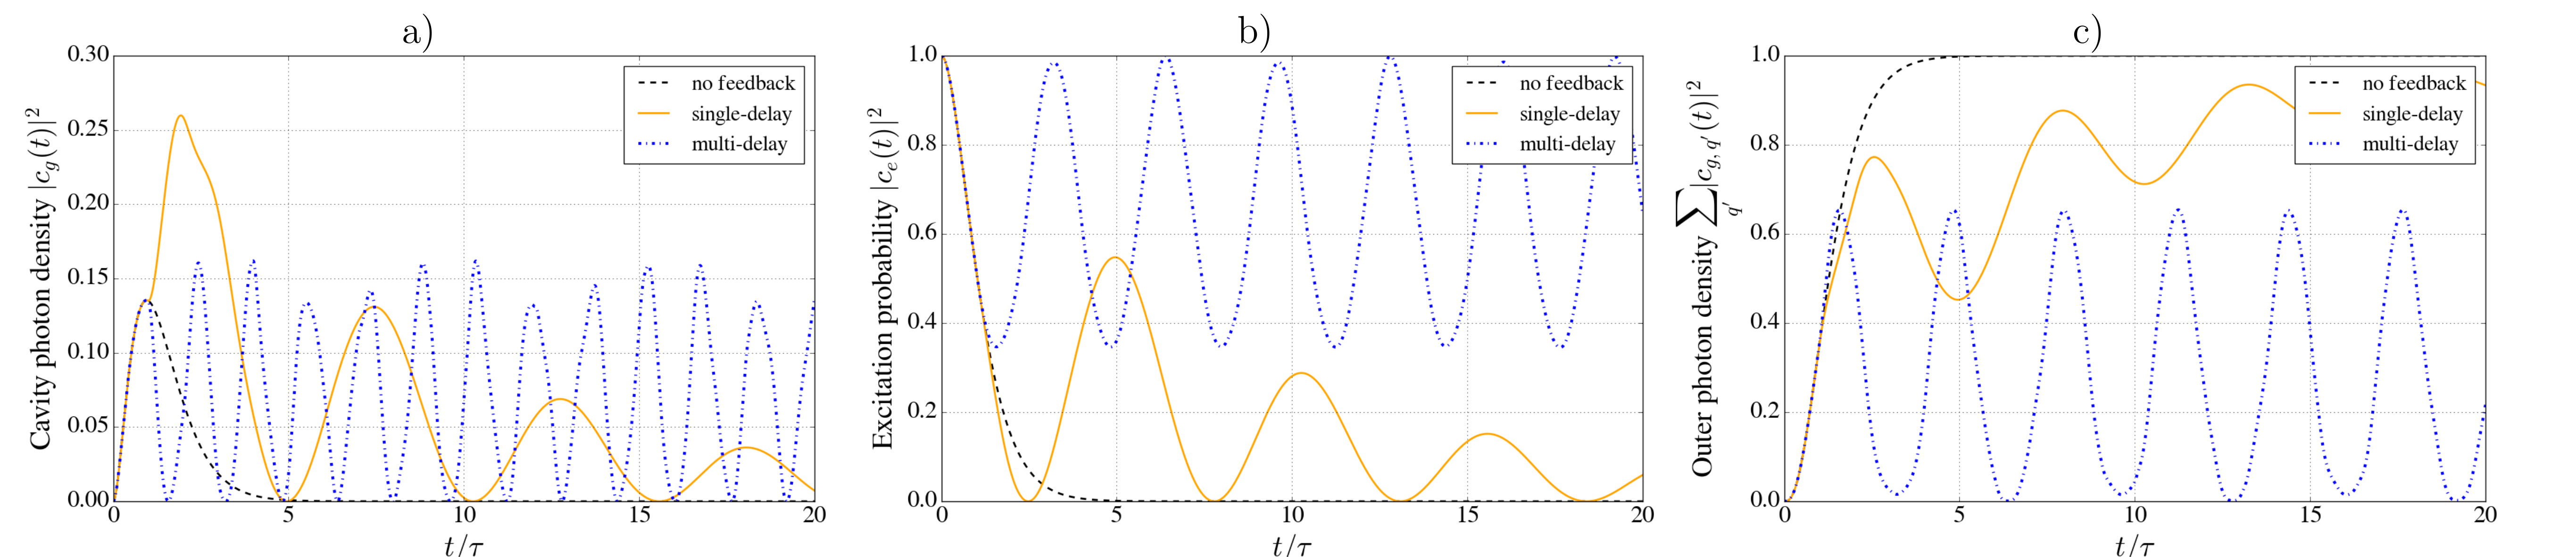
\includegraphics[width=1.05\textwidth]{longtime_kap=2,gam=1,tau=pip3.png}
\vglue -1 cm
\label{fig:weak_envtls}
\textit{\textbf{\caption{\linespread{1}\small{Time-evolution of different excitation probabilities, when $\gamma=\kappap, \tau=\pi/3\gamma$ in the long-time limit. The single-delay case is calculated from \cite{Kabuss2015}.}}}}
\vglue -.4 cm
\end{figure}

\newpage
\subsection{Strong-coupling regime}
Similar features as the Rabi oscillations can be recovered for a certain value of time-delay
\begin{figure}[h!]
\centering
\vglue -.35 cm
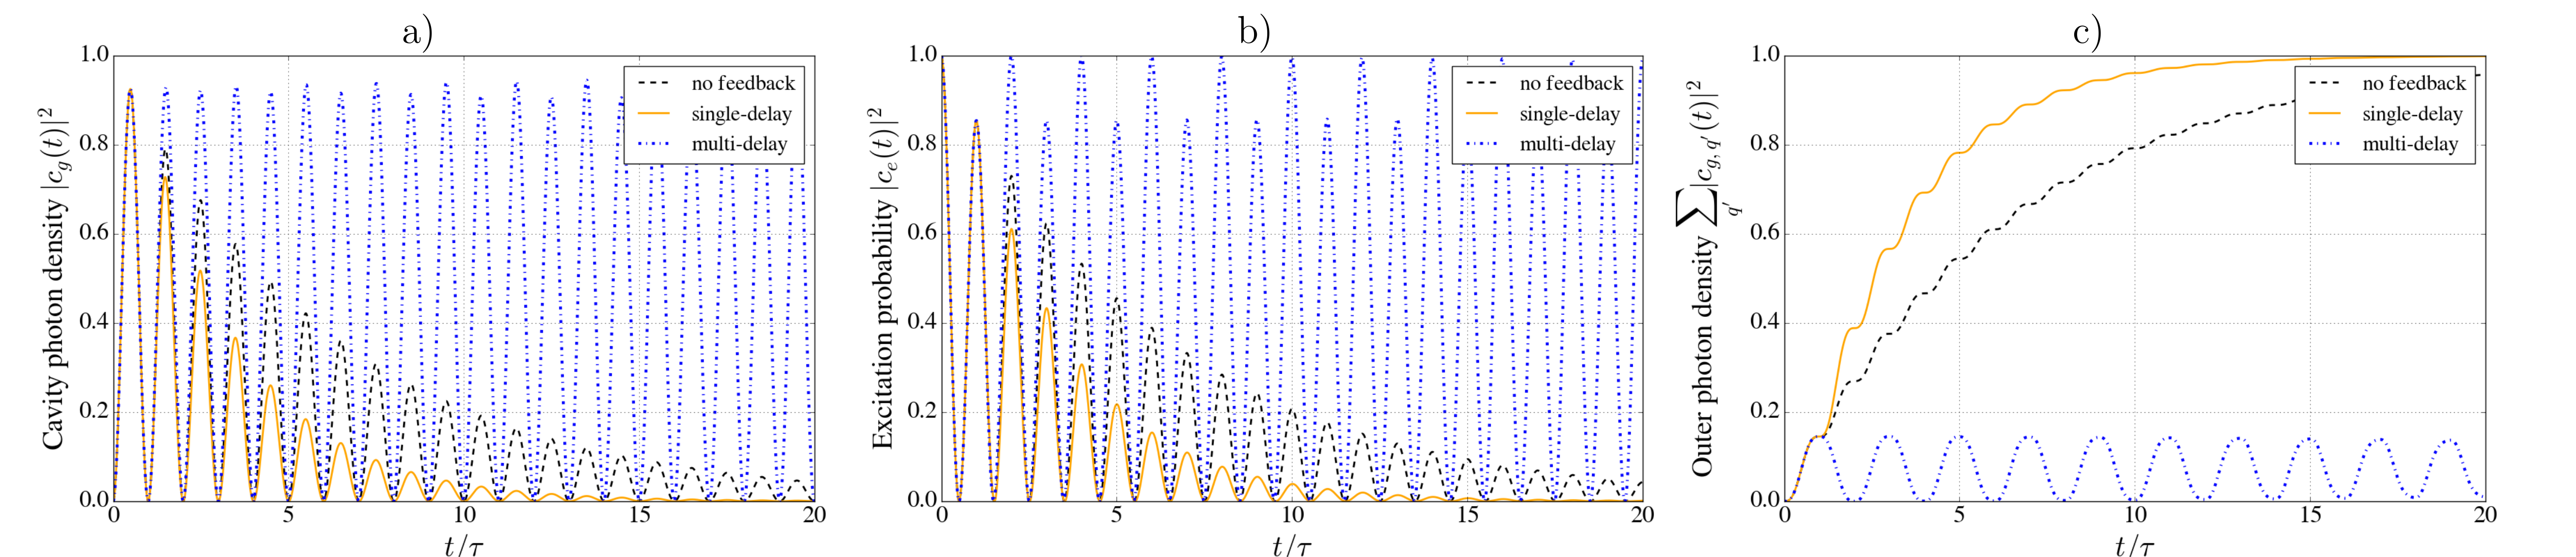
\includegraphics[width=1.05\textwidth]{longtime_kap=2,gam=40,tau=pip40.png}
\vglue -1 cm
\label{fig:strong_cavtls}
\textit{\textbf{\caption{\linespread{1}\small{Time-evolution of different excitation probabilities, when $\gamma=40\kappap, \tau=\pi/\gamma$ in the long-time limit. The single-delay case is calculated from \cite{Kabuss2015}.}}}}
\vglue -.1 cm
\end{figure}

\subsection{Continuous limit}
If the mirror is far enough, the field leaving the cavity behaves as a wave-packet that travels to the mirror and returns instead of interfering with itself. We can see signatures of such behaviour, when $\tau\approx 5\pi$, but it becomes completely clear at $\tau\approx 100\pi$.

\begin{figure}[h!]
\centering
\vglue -.2 cm
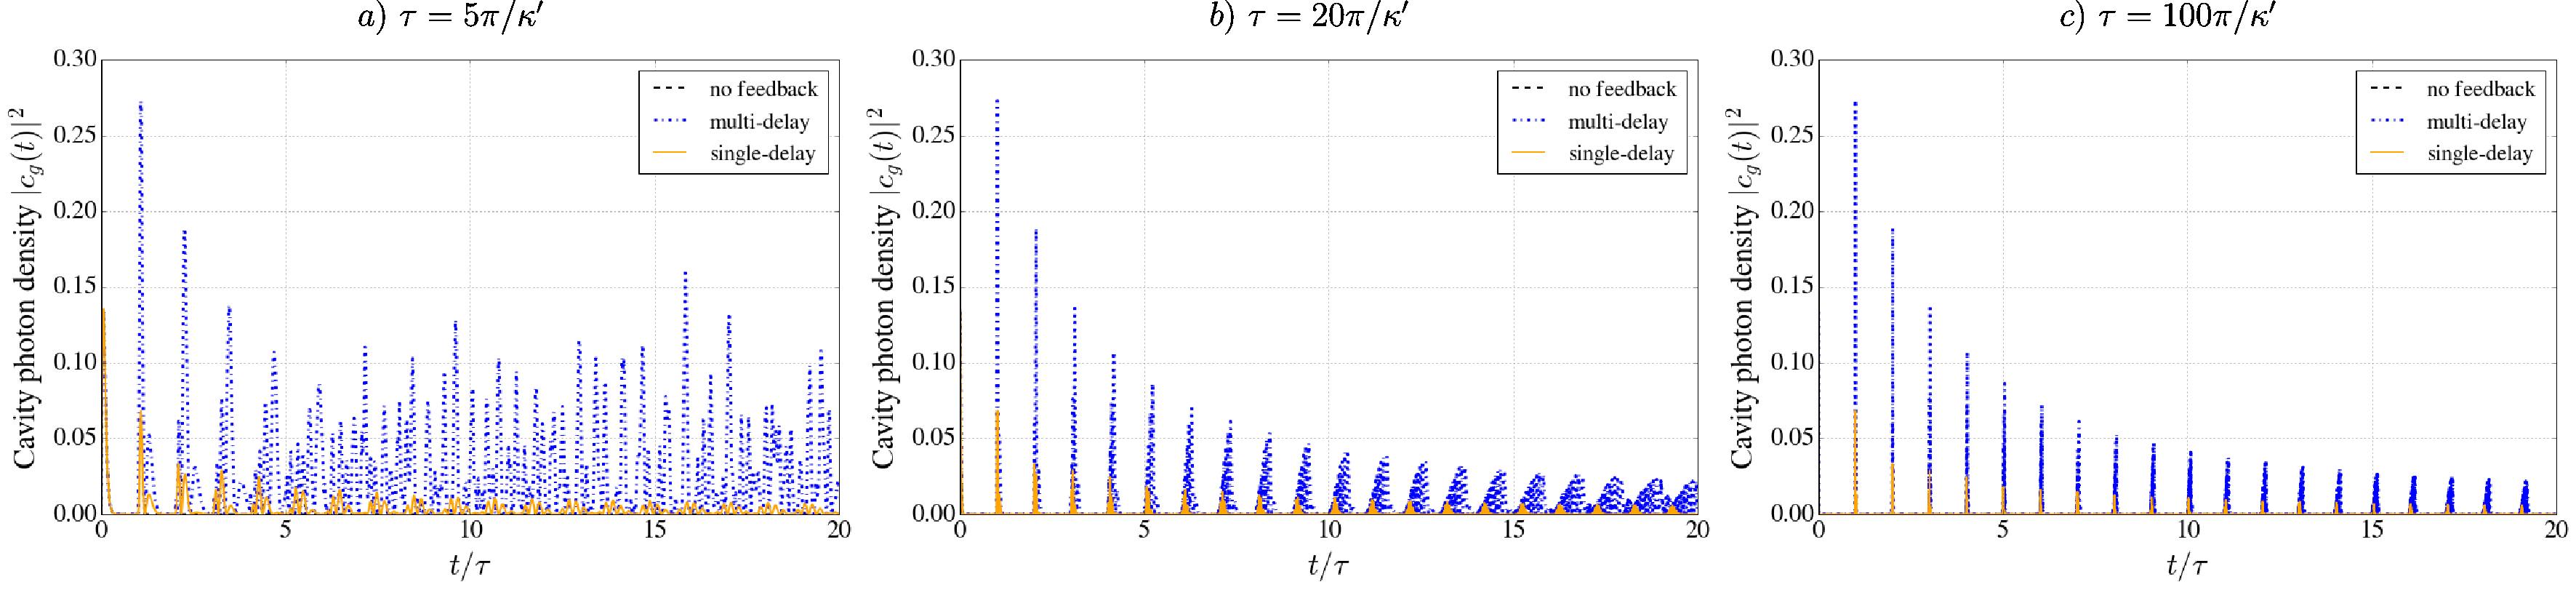
\includegraphics[width=1.0\textwidth]{longdelay_gam=kap=1.png}
\vglue -1 cm
\label{fig:strong_cavtls}
\textit{\textbf{\caption{\linespread{1}\small{Time-evolution of the cavity field for different length of time-delay, when $\gamma=\kappap=1\cdot 2\pi MHz$. The single-delay case is calculated from \cite{Kabuss2015}.}}}}
\vglue -.1 cm
\end{figure}

\begin{figure}[h!]
\centering
\vglue -.2 cm
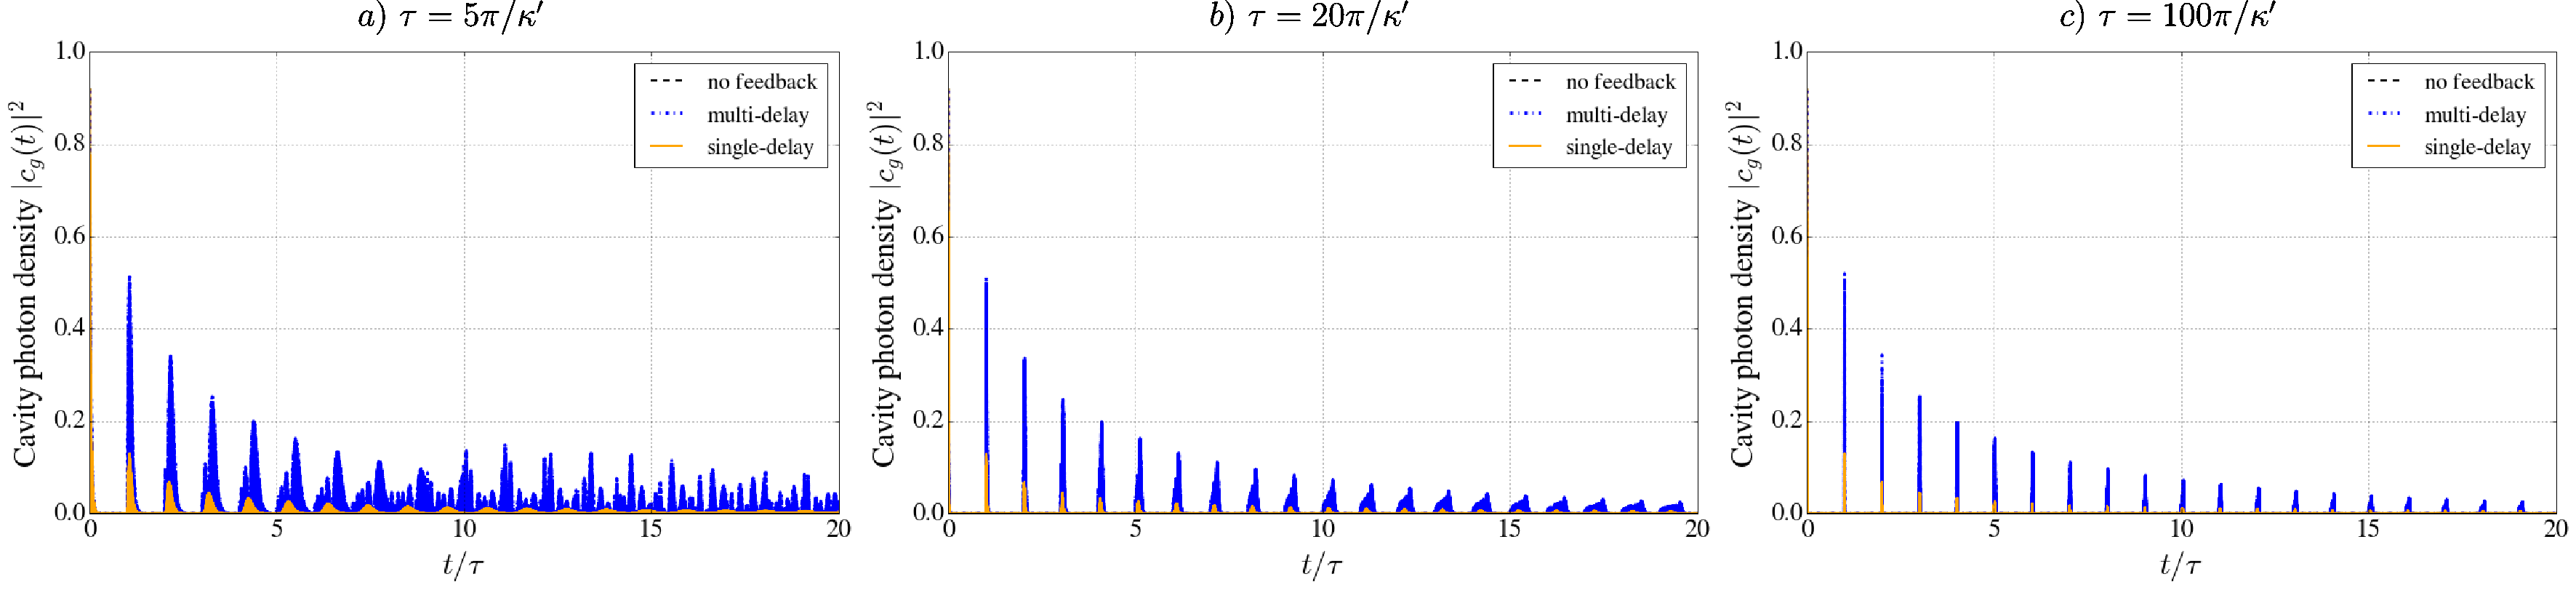
\includegraphics[width=1.0\textwidth]{longdelay_gam=40,kap=1.png}
\vglue -1 cm
\label{fig:strong_cavtls}
\textit{\textbf{\caption{\linespread{1}\small{Time-evolution of the cavity field for different length of time-delay, when $\gamma=40\kappap=40\cdot 2\pi MHz$. The single-delay case is calculated from \cite{Kabuss2015}.}}}}
\vglue -.1 cm
\end{figure}

One can zoom in to the individual peaks and compare the single-delay and multi-delay case at different times. For a weak coupling, the oscillations have the same frequency, there is only a difference in their intensity. However, for strong coupling, it looks as if in the multi-delay case the pulses reenterig the cavity after each roundtrip are not entering at the same time.

\begin{figure}[h!]
\centering
\vglue -.2 cm
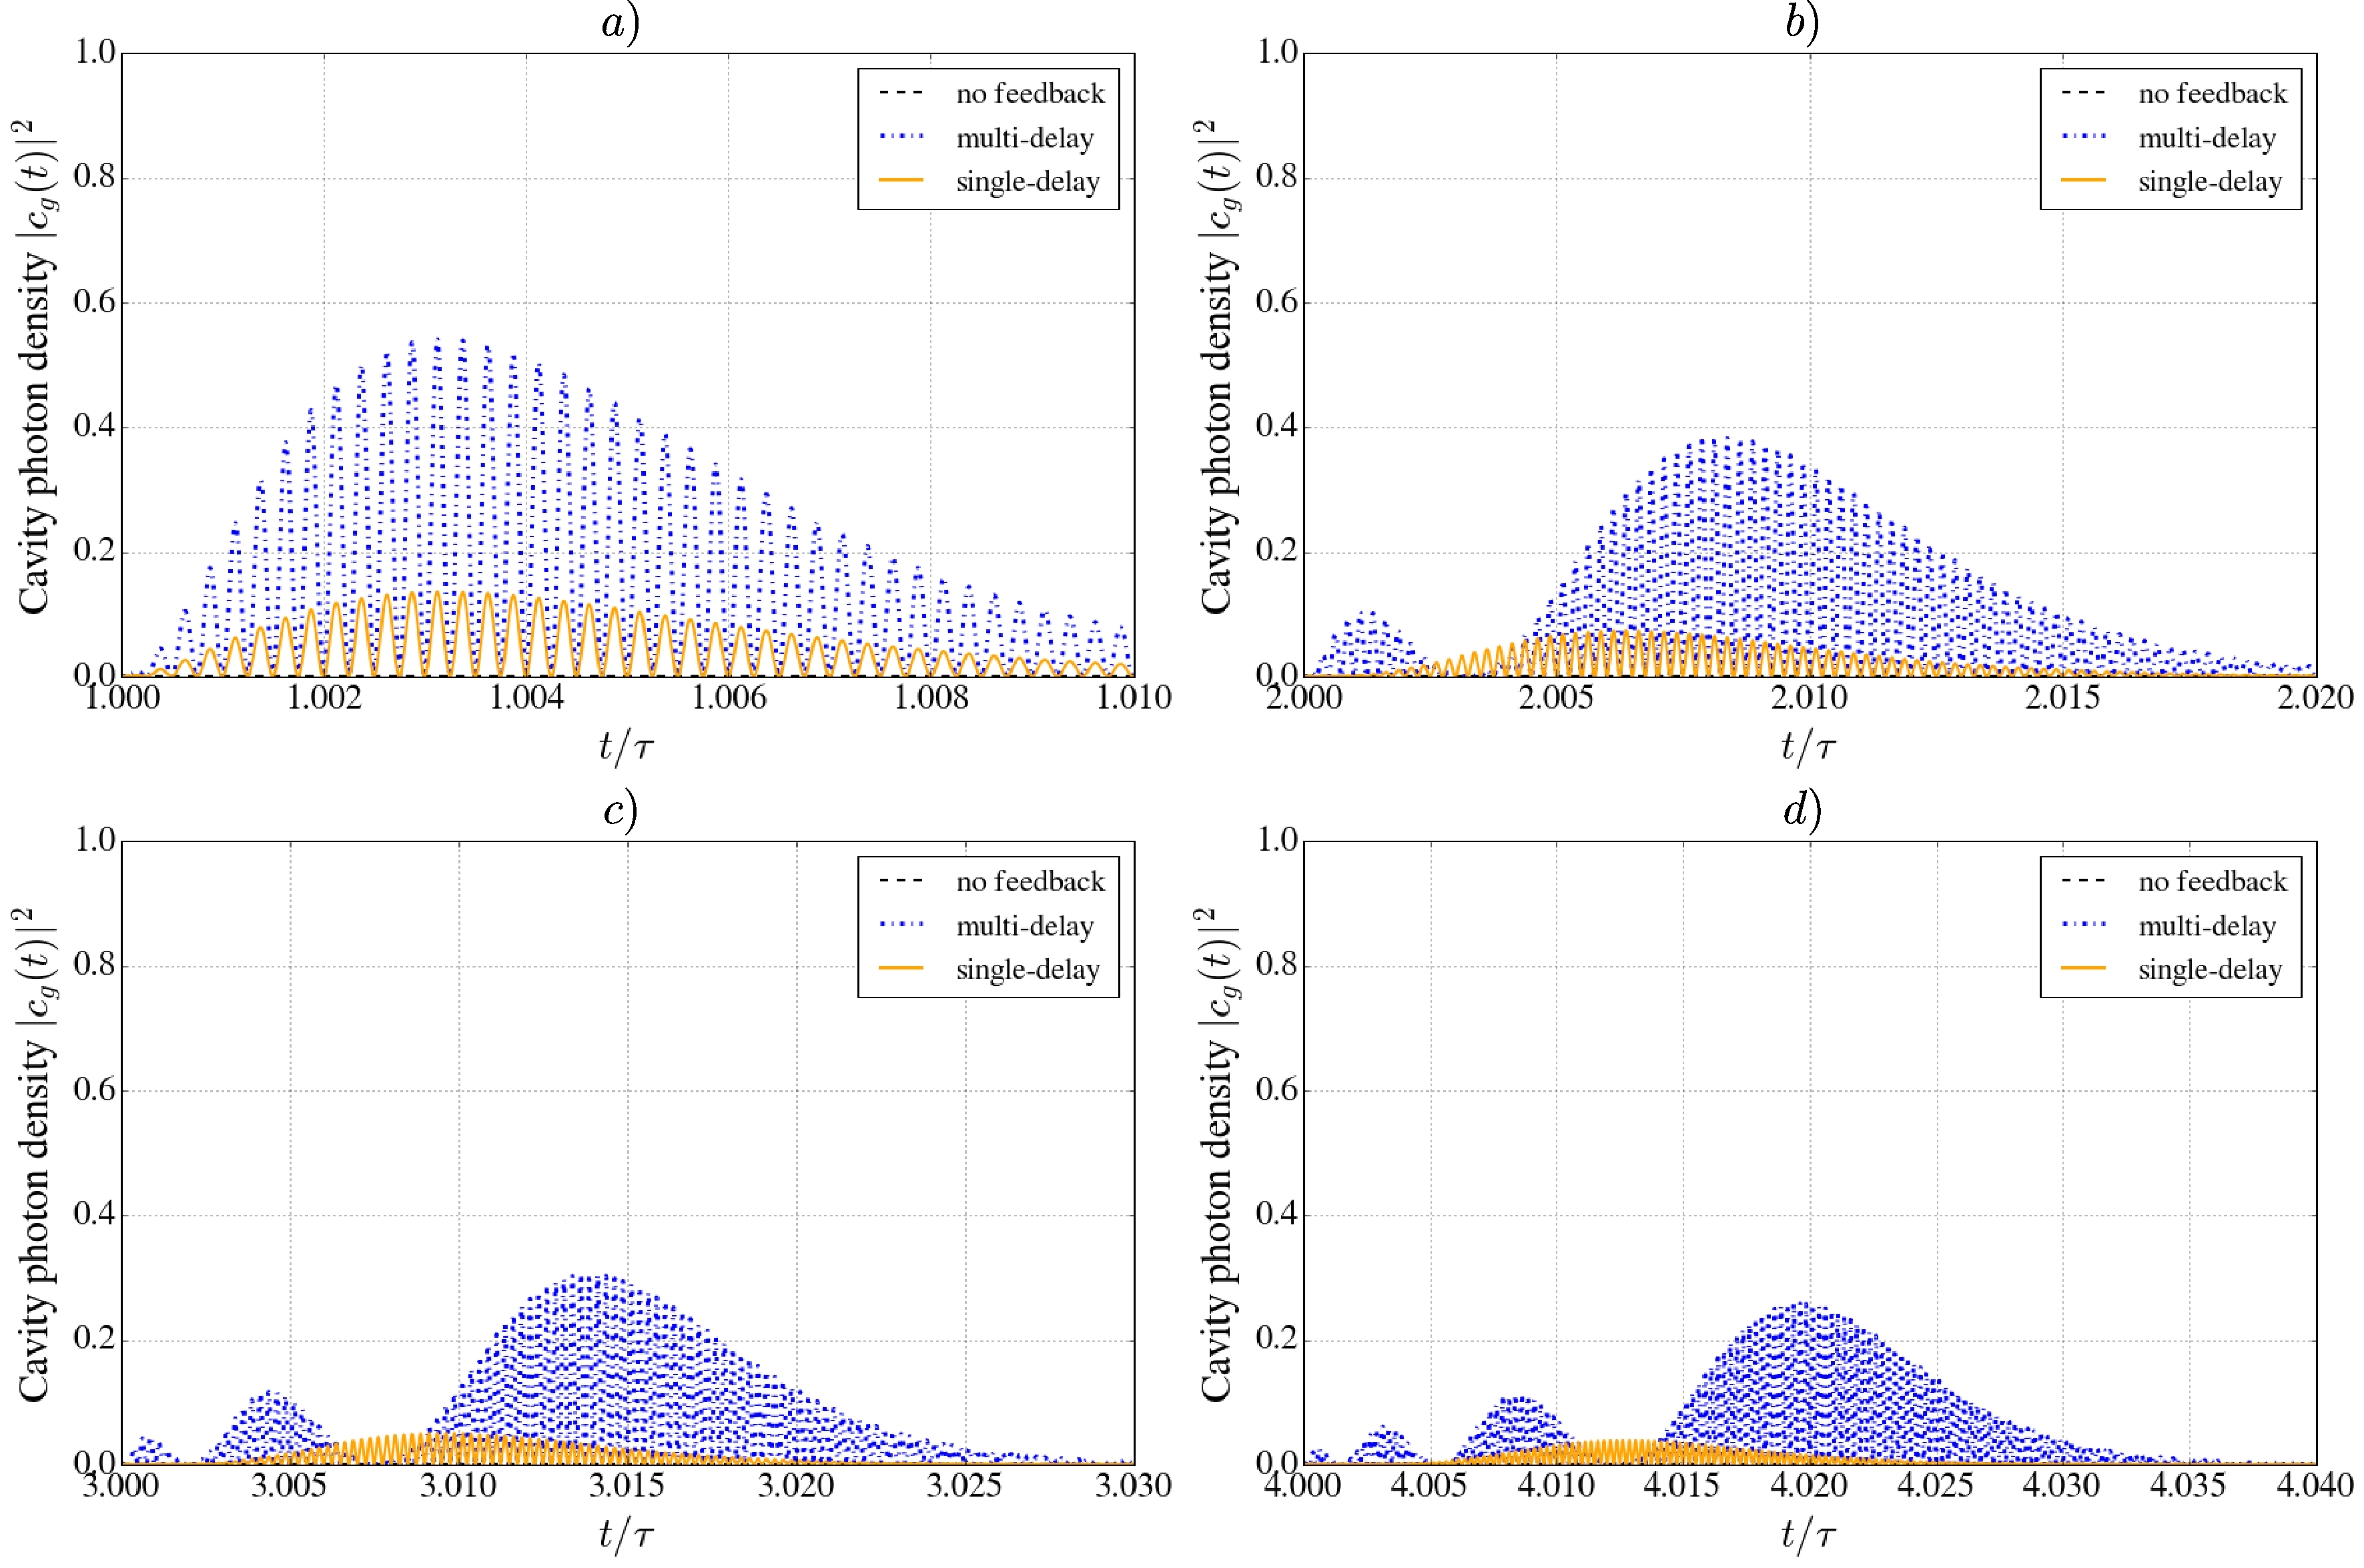
\includegraphics[width=0.8\textwidth]{longdelay_tau=100pi,kap=gam=1.png}
\vglue -1 cm
\label{fig:strong_cavtls}
\textit{\textbf{\caption{\linespread{1}\small{Different sections of the time-evolution of the cavity field for different length of time-delay, when $\gamma=\kappap=1\cdot 2\pi MHz,\kappa\tau = 100\pi$. The single-delay case is calculated from \cite{Kabuss2015}.}}}}
\vglue -.1 cm
\end{figure}

\begin{figure}[h!]
\centering
\vglue -.2 cm
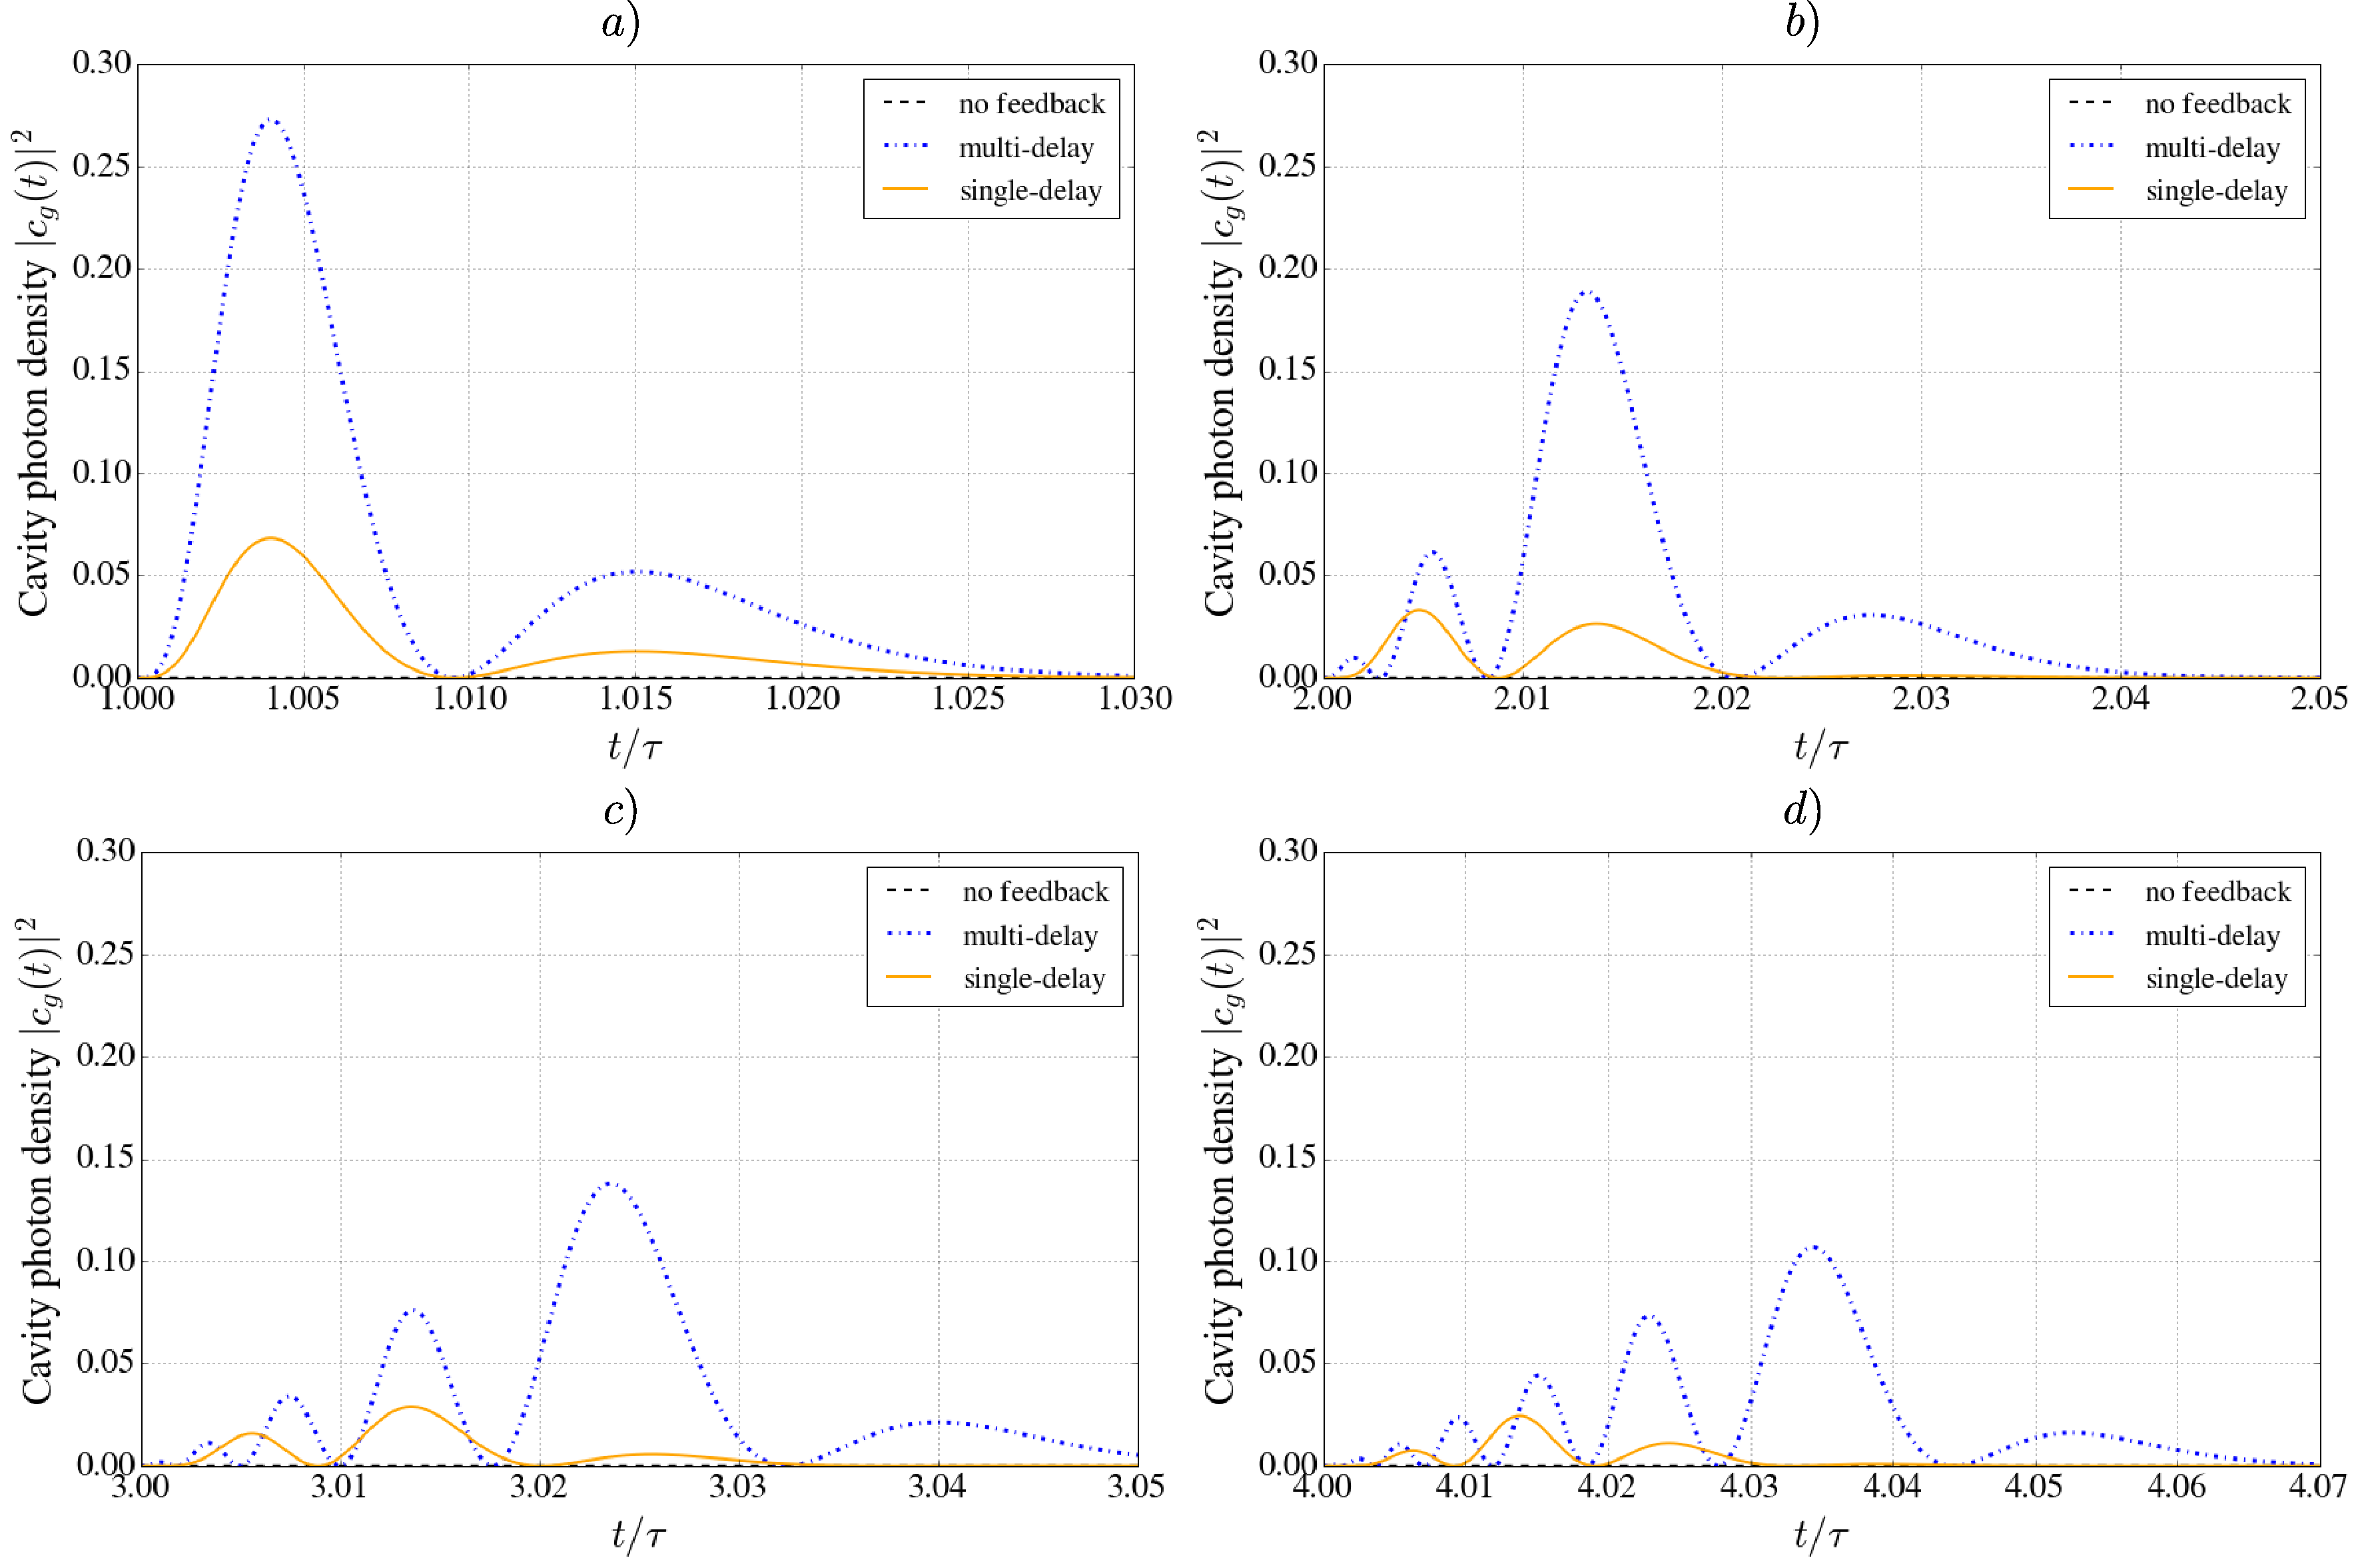
\includegraphics[width=0.8\textwidth]{longdelay_tau=100pi,kap=1,gam=40.png}
\vglue -1 cm
\label{fig:strong_cavtls}
\textit{\textbf{\caption{\linespread{1}\small{Different sections of the time-evolution of the cavity field for different length of time-delay, when $\gamma=40\kappap=40\cdot 2\pi MHz,\kappa\tau = 100\pi$. The single-delay case is calculated from \cite{Kabuss2015}.}}}}
\vglue -.1 cm
\end{figure}


\newpage
\begin{align*}
\
\end{align*}

\newpage
\subsection{Damped system}
One can introduce an output channel at the other side of the cavity, where a detector can be placed. In this case an additional $-\kappa_1c_g(t)$ term should be added to the equation of motion \refeq{c_g_eq}. The previous amplitude evolutions are modified as follows:
\begin{figure}[h!]
\centering
\vglue -.2 cm
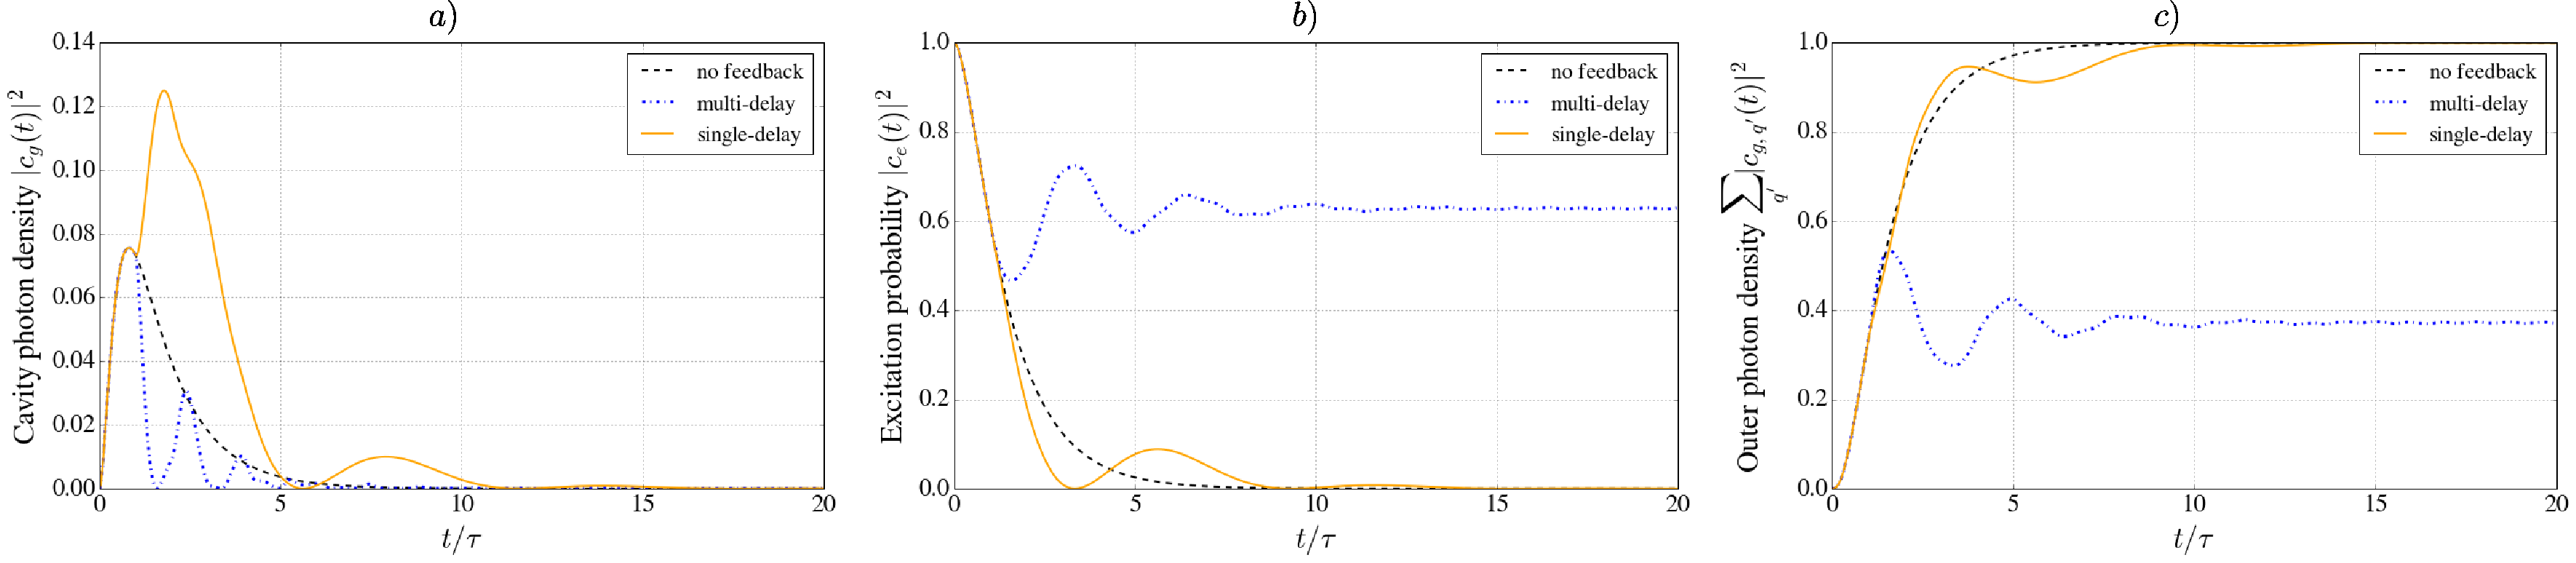
\includegraphics[width=0.8\textwidth,trim={0 0 10cm 0},clip]{longtime_kapp=1,kap=2,gam=1,tau=pip3.png}
\vglue -1 cm
\label{fig:strong_cavtls}
\textit{\textbf{\caption{\linespread{1}\small{Time-evolution of the cavity density and atomic excitation in a damped system, when $\gamma=\kappap=\kappa_1=1\cdot 2\pi MHz$. The single-delay case is calculated from \cite{Kabuss2015} with the extra damping term.}}}}
\vglue -.2 cm
\end{figure}

\begin{figure}[h!]
\centering
\vglue -.2 cm
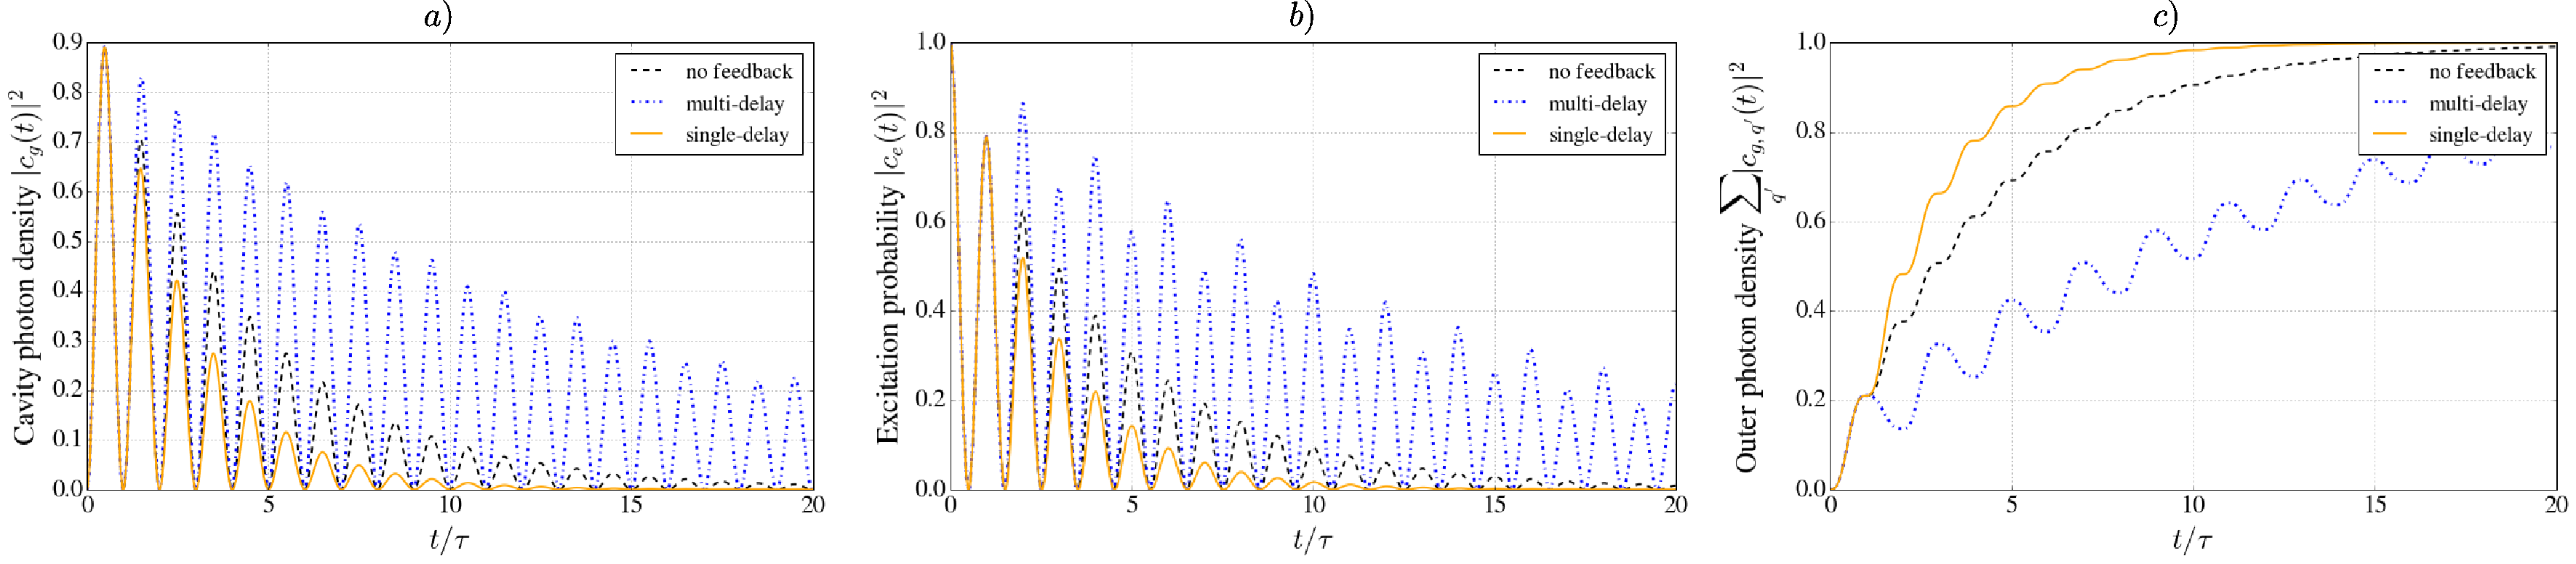
\includegraphics[width=0.8\textwidth,trim={0 0 10cm 0},clip]{longtime_kapp=1,kap=2,gam=40,tau=pip40.png}
\vglue -1 cm
\label{fig:strong_cavtls}
\textit{\textbf{\caption{\linespread{1}\small{Time-evolution of the cavity density and atomic excitation in a damped system, when $\gamma=40\kappap=40\kappa_1=40\cdot 2\pi MHz$. The single-delay case is calculated from \cite{Kabuss2015} with the extra damping term.}}}}
\vglue -.1 cm
\end{figure}

\subsubsection{Spontaneous emission spectra}
The Laplace transform of the cavity field derived from the time-local system of equations \refeq{c_e_eq}-\refeq{c_gqp_eq} with the extra damping term:
\begin{align}
\tilde{c}_g^{(TL)}(s) = i\gamma\lsz s^2+\gamma^2+\kappa_1s+4\kappap s\sum_{\qp=-\frac{N-1}{2}}^{\frac{N-1}{2}}\frac{1}{s\tau+i2\qp\pi}\rsz^{-1},
\end{align}
where we consider only $N$ number of modes, which are the closest to the cavity resonance. 

From the delayed model, described by Laplace transforms \refeq{eq:lap_ce} and \refeq{eq:lap_cg} we obtain in the damped case:
\begin{align}
\ctil(s) = i\gamma\lsz s^2+\gamma^2+\kappa_1s + 4\kappap s\lk\sum_{\qp=0}^\infty e^{-s\qp\tau}-\frac{1}{2}\rk\rsz^{-1}
\end{align}
The sum in this expression is convergent if $s$ has a real part. 
The spontaneous emission spectra can be expressed as:
\begin{align}
S(\omega) = \frac{\kappa_1}{2\pi}
\end{align}
The obtained spontaneous emission spectra for the weak coupling case:
\begin{figure}[h!]
\centering
\vglue -.2 cm
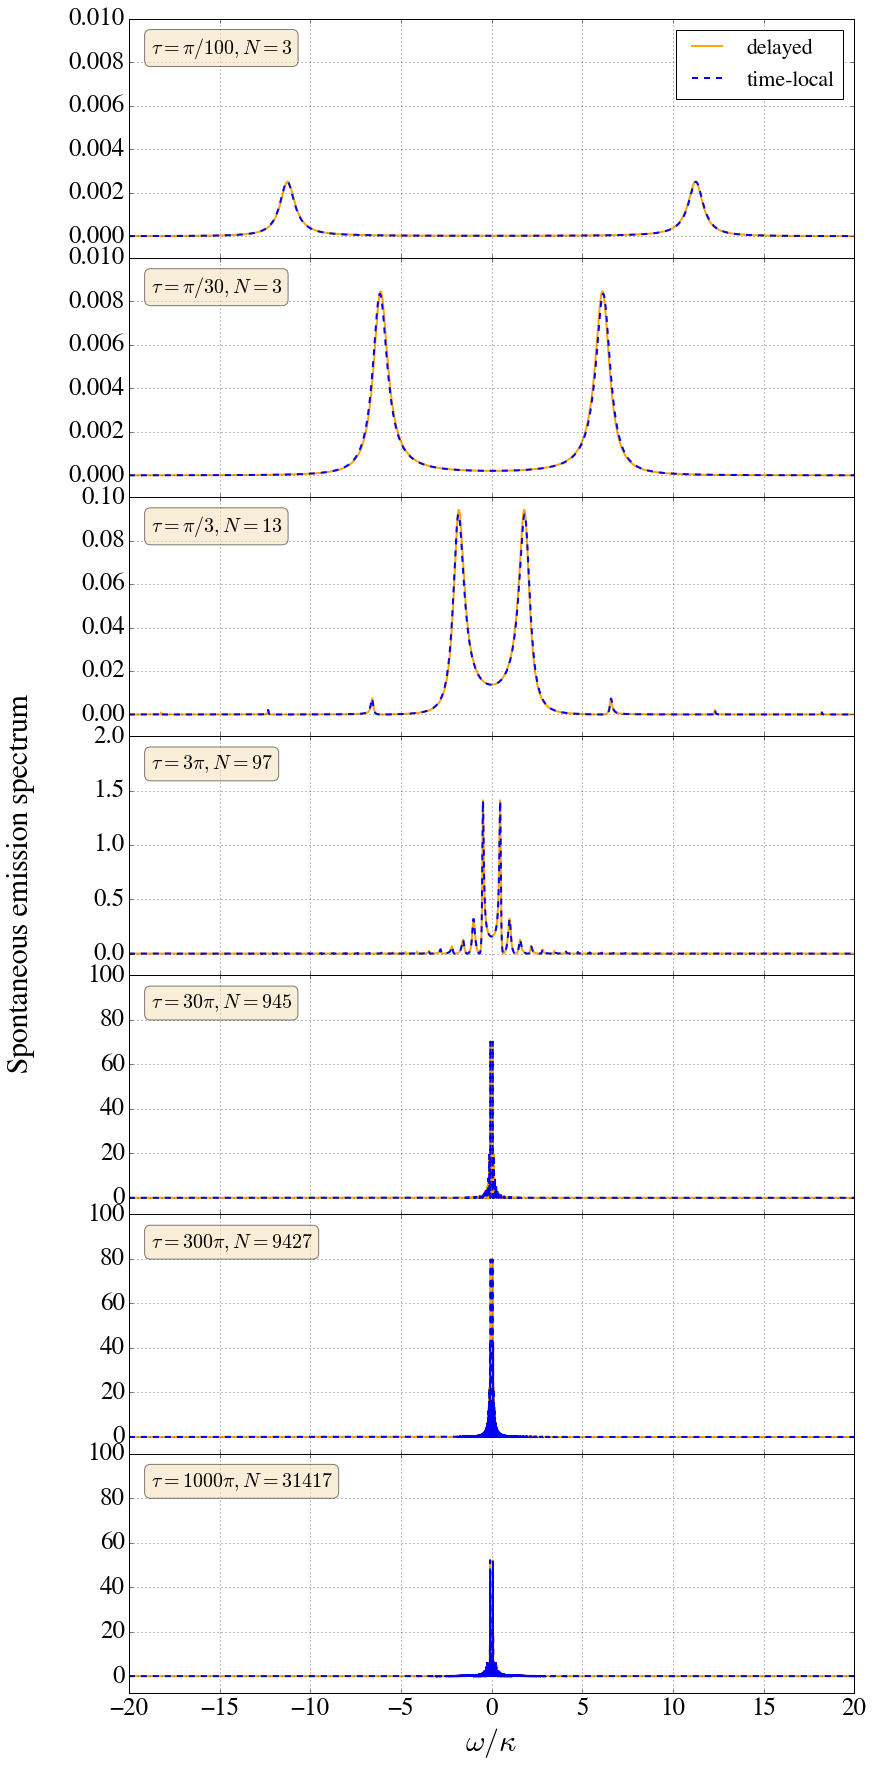
\includegraphics[width=0.5\textwidth]{Spontem_kap=kap1=gam=1.png}
\vglue -1 cm
\label{fig:strong_cavtls}
\textit{\textbf{\caption{\linespread{1}\small{Spontaneous emission spectra through the cavity mirror, when $\gamma=\kappap=\kappa_1=1\cdot 2\pi MHz$.}}}}
\vglue -.1 cm
\end{figure}

\newpage
In the weak coupling case the two theories agree well in most of the cases. However, in the strong coupling case, there are differences in the spectra.
\begin{figure}[h!]
\centering
\vglue -.2 cm
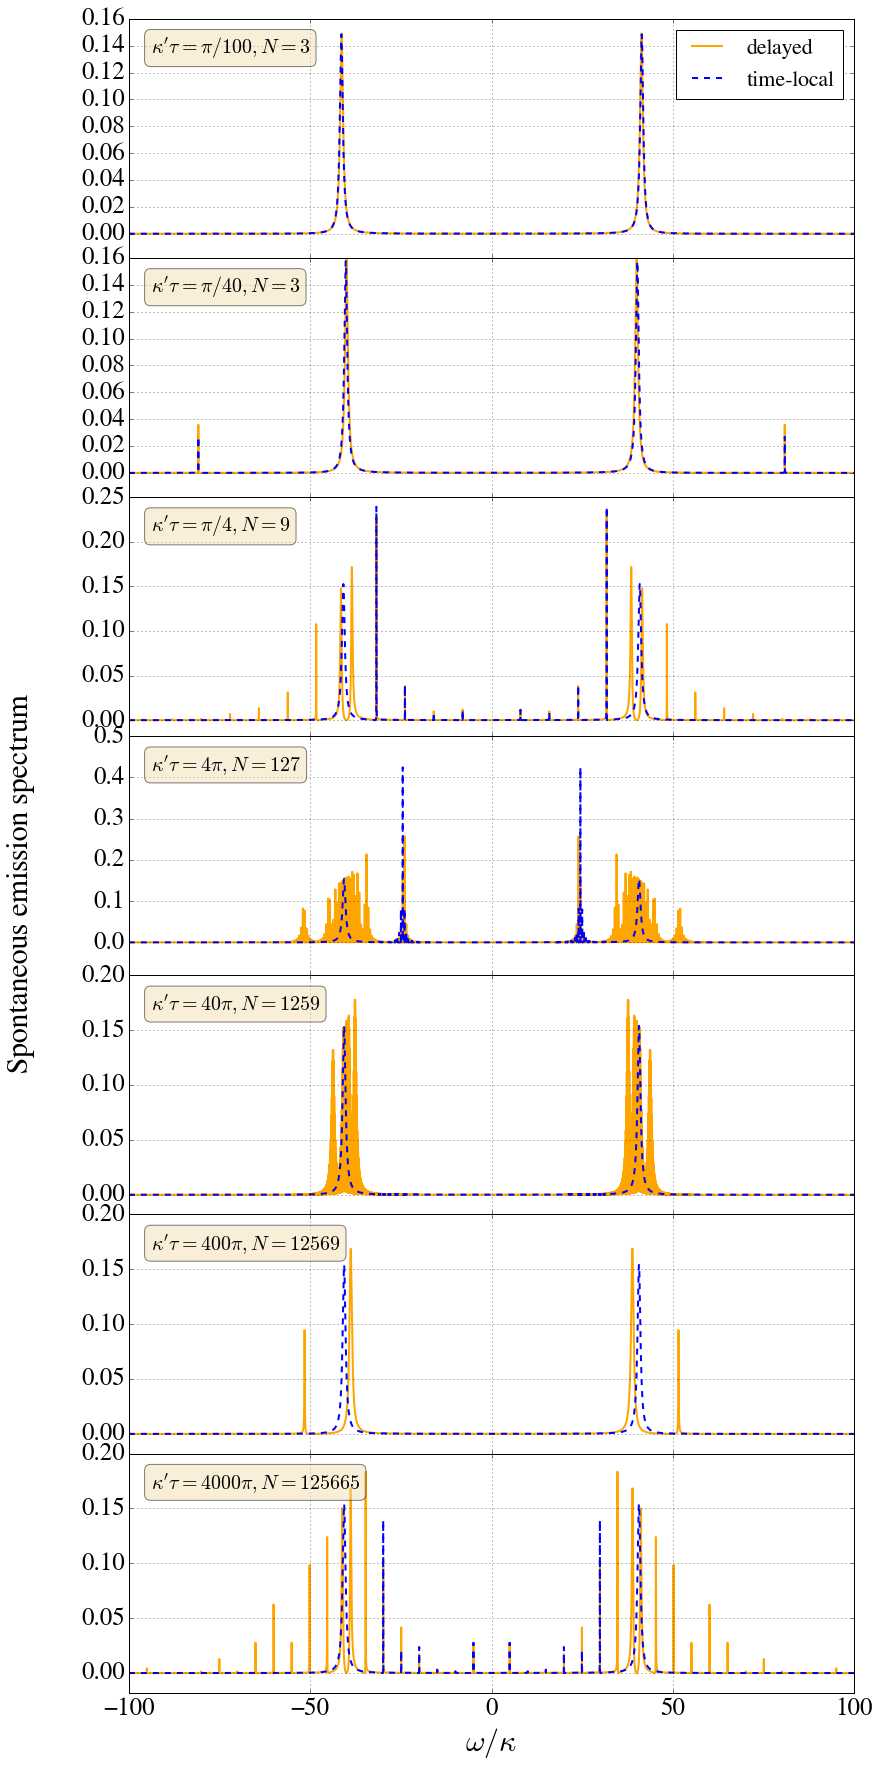
\includegraphics[width=0.5\textwidth]{Spontem_kap=kap1=1,gam=40.png}
\vglue -1 cm
\label{fig:strong_cavtls}
\textit{\textbf{\caption{\linespread{1}\small{Time-evolution of the cavity density and atomic excitation in a damped system, when $\gamma=40\kappap=40\kappa_1=40\cdot 2\pi MHz$. The single-delay case is calculated from \cite{Kabuss2015} with the extra damping term.}}}}
\vglue -.4 cm
\end{figure}




\begin{thebibliography}{9}
\bibitem{Kabuss2015} 
J. Kabuss, D.~O. Krimer, S. Rotter, K. Stannigel, A. Knorr and A. Carmele. Analytical study of quantum-feedback-enhanced Rabi oscillations, PRA {\bf 92}, 053801 (2015)
\bibitem{Dorner2002} 
U. Dorner and P. Zoller. Laser-driven atoms in half-cavities, PRA {\bf 66}, 023816 (2002)

\end{thebibliography}
\end{document}
